\interfootnotelinepenalty=10000

\chapter{Multi-speaker localization}
\label{chap:multisourceLocalization}

\lettrine{I}{n} Chapter~\ref{chap:tdvv}, we explored single-speaker localization with a novel type of input feature called TDVV. We now focus on multi-speaker localization. However, TDVV assumes a single sound source, hence we will rely on the pseudointensity vector (which way, anyhow, shown to outperform the former even in the single-source scenario). We base our research on the same baseline \cite{perotin_crnn-based_2019} as in Chapter~\ref{chap:tdvv}, and propose to improve several components of this system. In the present chapter, the NoS is supposed to be known by the localization system.

After describing the neural network input features, the output paradigm and overall architecture, we present different parameters used in our system, the employed training and testing data, the baseline and evaluation metrics. Then, we detail the various experiments we conduct to improve the multi-speaker localization performance over the baseline. The first experiment aims at finding the best order of feeding the training data to the network, considering that the training signals contains between $1$ and $3$ speakers. In the second experiment, we design a new feature extraction module, and in the third, we consider replacing the recurrent layers with a self-attention mechanism. In the last experiment, we assess the use of HOA features.

%-----------------------------------------------
%  METHODOLOGY
%-----------------------------------------------
\section{Overall methodology}
\subsection{Input features}

As in \cite{perotin_crnn-based_2019}, we use the pseudointensity vector as input feature for the multi-speaker localization neural network. This type of input features proved to be more robust than spectrograms for FOA signals \cite{perotin_crnn-based_2018}. In \cite{perotin_crnn-based_2019}, the input feature was obtained by computing the normalized active and reactive FO-PIV $\bar{\mathbf{I}}_a(t,f)$ and $\bar{\mathbf{I}}_r(t,f)$ from \eqref{eq:activeFOPIV} and \eqref{eq:reactiveFOPIV} and stacking them into the third dimension to obtain a 3D tensor of shape $T \times F \times 6$, with $T$ the number of frames, $F$ the number of frequency bins.

Fig.~\ref{fig:foaIntensityVector} shows the input feature extracted from a training example. Here we have $T = 25$ frames, and $F=512$ frequency bins corresponding to the bandwidth $0-8$~kHz.

\begin{figure}[ht]
    \begin{adjustbox}{width=1.3\textwidth,center}
        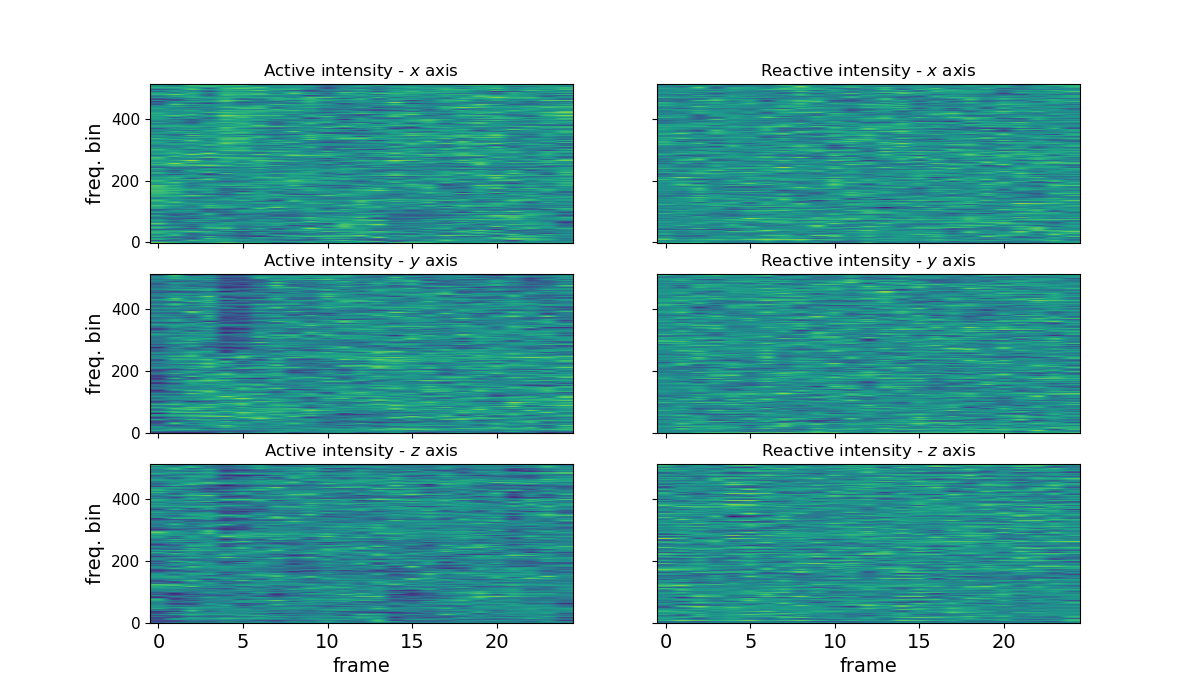
\includegraphics[width=1.\linewidth]{Images/chap7/foaIntensityVector.png}
    \end{adjustbox}
    \captionof{figure}[Plot of a FO-PIV feature of several frames]{Plot of the 6 channels of a FO-PIV input feature extracted from a training example of $25$ frames. From top to bottom: the $x$, $y$, $z$ coordinates. Left: active intensity. Right: reactive intensity.}
    \label{fig:foaIntensityVector}
\end{figure}

An extension of this input feature is assessed in an experiment presented in Section~\ref{ss:hoaExperiment}, in which we evaluate the benefit of using the HO-PIV over the FO-PIV. The HO-PIV feature is computed at order $2$, leading to an input tensor of shape $T \times F \times 16$.

\subsection{Multi-speaker localization as classification}
\label{ss:multiLocaClassif}

We consider the multi-speaker localization problem with the same classification approach as that described in Chapter~\ref{chap:tdvv} and illustrated in Fig.~\ref{fig:multiLocalizationClassification}. The same unit sphere discretization is used, leading to $429$ possible DoA directions, considered as classes. We extend SSL to the multi-speaker case by directly extracting the $J$ highest peaks in the output probability distribution, where $J$ is the number of speakers.
Note that, after averaging the probability distribution over the $T$ frames (which leads us to consider the total NoS $J$ instead of the instantaneous NoS $J(t)$), we do not smooth this probability distribution within a neighborhood like in \cite{perotin_crnn-based_2019}, as we found out it deteriorated the results.

When training and evaluating the network with generated data (using simulated and real SRIRs), we consider that $J$ is known. For the evaluation on real signals from the LOCATA dataset \cite{evers_locata_2020}, we use a thresholding method with a fixed threshold $\beta = 0.2$ for peak extraction.

When a certain number of DoAs are extracted from the localization network output, we employ the Hungarian algorithm \cite{kuhn_hungarian_1955} to assign the estimated DoAs with the ground-truth speaker positions. This algorithm minimizes the total assignment cost, as a sum of the costs obtained by the different assigned pairs. In the present case, it minimizes the total angular error obtained between all assigned pairs \{predicted source DoA, ground-truth source DoA\}.

\subsection{Neural network architecture}

\begin{figure}[ht]
    \begin{center}
    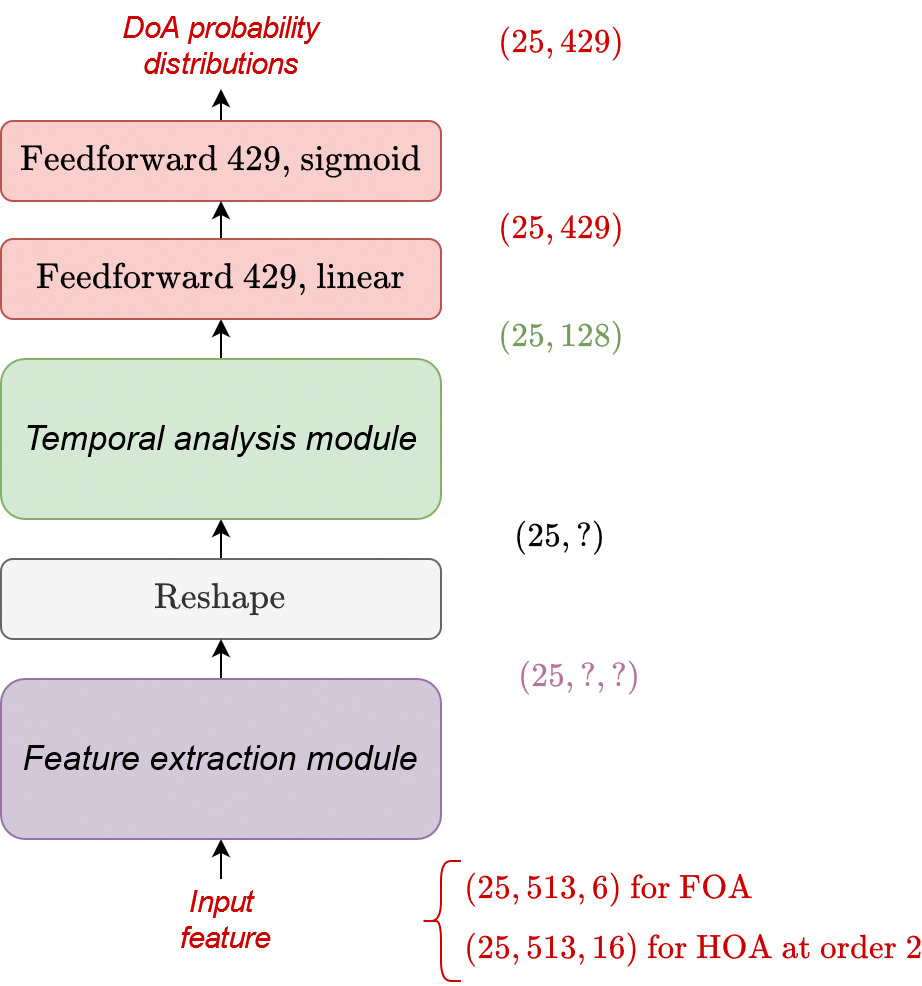
\includegraphics[width=0.7\linewidth]{Images/chap7/generalMultiLocalizationNetwork.png}
    \captionof{figure}[General architecture of the multi-speaker localization neural network]{General architecture of the multi-speaker localization neural network. The design of the feature extraction and temporal analysis modules are part of the experiments.}
    \label{fig:generalMultiLocalizationNetwork}
    \end{center}
\end{figure}

The general architecture for our multi-speaker localization system is shown in Fig.~\ref{fig:generalMultiLocalizationNetwork}. The input feature is first fed into a feature extraction module, whose design is addressed in our the second experiment in Section~\ref{ss:multiLocalizationfeatureExtractionModule} (in our first experiment in Section~\ref{ss:trainingOrder}, the feature extraction module architecture is the same as in the baseline). Then, the new extracted feature is reshaped and sent through the temporal analysis module. The temporal analysis module design is addressed in our third experiment in Section~\ref{ss:multiLocalizationSelfAttention}. Then, each vector of the output sequence of this temporal analysis module finally goes separately into the output feedforward layer, which produces a probability distribution over the DoA space. Note that throughout the whole architecture, the temporal dimension is preserved, so that the output sequence is of the same length as the input sequence.

As the reader will understand further in this chapter, we successively focused on different parts of this network architecture, \emph{i.e.}, the feature extraction module, the temporal analysis module, and the input feature, and experimented several changes to improve the localization performance over the baseline, which we detail below.

%-----------------------------------------------
% EXPERIMENTAL PROTOCOL
%-----------------------------------------------
\section{Experimental protocol}
\subsection{Audio and training parameters}

The same audio parameters as in Chapter~\ref{chap:tdvv} are used, except that the STFT is computed with a sinusoidal window, as in \cite{perotin_crnn-based_2019}. The training parameters are exactly the same. We consider $T=25$ frames for each input sequence. To train the network, we use the binary cross-entropy as in Chapter~\ref{chap:tdvv}.

\subsection{Training data}

The training dataset is generated in the same manner as the training data for the single-speaker localization system described in Chapter~\ref{ss:tdvvTrainingData}. The difference is that, when a first random DoA is picked, and the room configuration and microphone position are drawn, two other source DoAs are randomly picked so that the sources are in the room and their positions are at least $10$\textdegree apart from one another. We thus obtain $3$ SRIRs per room configuration and microphone position. This enables us to create $3$ distinct training datasets $T_1$, $T_2$, and $T_3$, which contain training signals with $1$, $2$, and $3$ speakers, respectively. This method follows the same protocol as in \cite{perotin_crnn-based_2019}, but is extended to $3$ speakers instead of $2$ as proposed by the authors of this study. For the training datasets $T_2$ and $T_3$, $1$-s single-speaker signals are first generated as in Section~\ref{ss:tdvvTrainingData}, by picking a distinct random SRIRs in the same room. They are then mixed together using random SIR in $[0,10]$~dB with respect to the first source (of course, we mix 2 signals for $T_2$, and we mix 3 signals for $T_3$).

At the end of this dataset generation process, the training datasets $T_1$, $T_2$, and $T_3$ each contain $257\,400$ $1$s-long mixtures (with $1$, $2$ and $3$ speakers, respectively), resulting in a total of $772\,200$ training mixtures (about $172$ hours of signals).

\subsection{Test data}

To evaluate our models, we use three sets of test data, each one of different nature. The first set is made of three datasets, labelled $E^{Sim}_1$, $E^{Sim}_2$ and $E^{Sim}_3$, which contain $1$-, $2$- and $3$-speaker signals, respectively. These signals are generated using the same simulated SRIRs as in Section~\ref{ss:tdvvTestData}, and are created in the same manner as for the training data with several speakers. The second set is also made of three datasets, named $E^{Real}_1$, $E^{Real}_2$ and $E^{Real}_3$, whose signals are generated using the same real SRIRs as in Section~\ref{ss:tdvvTestData} and the same process as the previously described multi-speaker mixtures. The third test dataset consists of the datasets of four tasks of the LOCATA Challenge \cite{evers_locata_2020}. These data are used to assess our model on real data. Focusing on the EigenMike signals of all these LOCATA datasets, we use $13$ signals of task 1 (single static loudspeaker), $13$ signals of task 2 (multiple static loudspeakers), $5$ signals of task 3 (single moving human talker) and $5$ signals of task 4 (multiple moving human talkers). Although we do not focus on moving speakers and our model is not trained for this scenario, we still perform an evaluation on task 3 and 4 to assess the robustness of our system to moving sources. These $4$ test datasets are referred as $E^{Rec}_1$, $E^{Rec}_2$, $E^{Rec}_3$ and $E^{Rec}_4$, for task 1, 2, 3 and 4, respectively.

\subsection{Baseline}

As a baseline, we use the same architecture as proposed in \cite{perotin_crnn-based_2019}, which is illustrated in Fig.~\ref{fig:perotinCRNN}. This baseline can be also described by Fig.~\ref{fig:generalMultiLocalizationNetwork} in which the feature extraction module contains three convolutional layers, each followed by a max-pooling layer, and the temporal analysis module is composed of two bidirectional LSTM layers. For fair comparison, we extend this model by training it with $3$-speaker signals, whereas the authors of \cite{perotin_crnn-based_2019} limited the training to $2$-speaker mixtures. For the last experiments, which assess the benefit of using HOA features, we also compare our system to an adaptation of a DL-free algorithm \cite{kitic_tramp:_2018}, called \textit{TRAMP}, to the same feature format. This method is based on the histogram of the DoAs derived from the pseudointensity vector over all considered frames and frequencies in the sequence.

\subsection{Evaluation metrics}

We use the same metrics as in Chapter~\ref{chap:tdvv}: the localization accuracy with an angular tolerance of $10$\textdegree~and $15$\textdegree, as well as a tolerance of $20$\textdegree~for the LOCATA dataset, and the mean and median angular errors.

%-----------------------------------------------
%  EXPERIMENTS
%-----------------------------------------------
\section{Experiments}

\subsection{Training scheme}
\label{ss:trainingOrder}
\subsubsection{Experiment objective}

As mentioned above, in the baseline study \cite{perotin_crnn-based_2019}, the experiments are limited to two speakers (thus, two training datasets), and during the training phase, the signals are fed into the network in a random order, regardless the number of speakers. This choice raises the question if there is an ``optimal'' order to present the training data to the neural network. One could think that the network is flexible enough to learn with all data mixed together, or on the contrary one could believe that it would be better for the network to be trained in an increasing order of complexity; that is, starting with signals with $1$ speaker, then $2$ speakers, and ending with $3$ speakers, which can be thought as fine-tuning. Another possibility is to train the network with $3$-speaker signals only (the most complex task), which may be enough to make the network robust for the easier tasks, \emph{i.e.}, localizing $1$ or $2$ speakers. This idea is actually linked to the concept of curriculum training \cite{bengio_curriculum_2009,jiang_self-paced_2015}.

In the present experiment, we assess these ideas by training the baseline neural network of \cite{perotin_crnn-based_2019} multiple times, using several training schemes and evaluating the obtained models on the test datasets $E^{Sim}_j$ and $E^{Real}_j$ for $j \in {1,2,3}$. The different training schemes we evaluate are the following:
\begin{itemize}
    \item The training is done with only one of the three training datasets $T_1$, $T_2$, or $T_3$. This enables us to determine how the neural network is able to adapt to simpler situations (\emph{e.g.}, when training on $T_3$ and evaluated on $E^{Sim}_1$) or more complex ones (\emph{e.g.}, when training on $T_1$ and evaluated on $E^{Sim}_3$). The models trained on $T_1$, $T_2$, and $T_3$ are labelled $M_{T_1}$, $M_{T_2}$, and $M_{T_3}$, respectively.
    \item The training is done with several datasets mixed together, as in \cite{perotin_crnn-based_2019}. In that case, the training examples are drawn randomly from all datasets. More specifically, we evaluate the model trained using $T_1$ and $T_2$, labelled as $M_{T_1 \bigcup T_2}$, and the one trained with all three datasets, labelled as $M_{T_1 \bigcup T_2 \bigcup T_3}$.
    \item The training is done in a sequential way, with the datasets presented one after another. The model is first trained with $T_1$ in a conventional manner (\emph{i.e.}, using early stopping by monitoring the validation accuracy and using a decreasing learning rate). When this first training is done, we refine the model by training it on $T_2$, starting with the weights from the training with $T_1$ (in short, training with $T_1$ and fine-tuning with $T_2$). Then, training is done with $T_3$. This method is intuited by the fact that the neural network is forced to learn the task from the easier to the most complex one. The model trained with $T_1$ then $T_2$ is labelled $M_{T_1 \rightarrow T_2}$, and the model trained with $T_1$, then $T_2$, and then $T_3$ is labelled $M_{T_1 \rightarrow T_2 \rightarrow T_3}$.
\end{itemize}

\subsubsection{Results}

\begin{table}[t]
\centering

    \subfloat[Simulated SRIRs]{
        \begin{adjustbox}{width=1.3\textwidth,center}
            \begin{tabular}{|c|cccc|cccc|cccc|}
            \hline
            \multirow{3}{*}{\textbf{Model label}}        & \multicolumn{4}{c|}{\textbf{$E^{Sim}_1$}}                                                        & \multicolumn{4}{c|}{\textbf{$E^{Sim}_2$}}                                                        & \multicolumn{4}{c|}{\textbf{$E^{Sim}_3$}}                                                         \\ \cline{2-13} 
                                                         & \multicolumn{2}{c}{\textbf{Accuracy (\%)}}     & \multicolumn{2}{c|}{\textbf{Angular error (°)}} & \multicolumn{2}{c}{\textbf{Accuracy (\%)}}     & \multicolumn{2}{c|}{\textbf{Angular error (°)}} & \multicolumn{2}{c}{\textbf{Accuracy (\%)}}     & \multicolumn{2}{c|}{\textbf{Angular error (°)}} \\
                                                         & \textbf{\textless 10°} & \textbf{\textless 15°} & \textbf{Mean}         & \textbf{Median}        & \textbf{\textless 10°} & \textbf{\textless 15°} & \textbf{Mean}         & \textbf{Median}        & \textbf{\textless 10°} & \textbf{\textless 15°} & \textbf{Mean}         & \textbf{Median}         \\ \hline
            \textbf{$M_{T_1}$}                               & \textbf{95.2}          & 99.1                   & \textbf{5.0}          & \textbf{4.5}           & 29.5                   & 40.1                   & 41.4                  & 23.1                   & 16.4                   & 26.3                   & 45.2                  & 34.0                    \\
            \textbf{$M_{T_2}$}                               & 91.8                   & 98.6                   & 5.8                   & 5.2                    & 76.3                   & 87.0                   & 12.0                  & 6.4                    & 45.9                   & 60.3                   & 25.6                  & 11.2                    \\
            \textbf{$M_{T_3}$}                              & 89.9                   & 98.1                   & 6.1                   & 5.4                    & 77.3                   & \textbf{87.9}          & 11.8                  & 6.4                    & \textbf{61.5}          & \textbf{75.6}          & \textbf{18.5}         & \textbf{8.0}            \\
            \textbf{$M_{T_1 \bigcup T_2}$}                   & 94.9                   & 99.0                   & 5.2                   & \textbf{4.5}           & \textbf{78.4}          & 87.1                   & \textbf{10.7}         & \textbf{5.9}           & 52.3                   & 65.3                   & 21.4                  & 9.4                     \\
            \textbf{$M_{T_1 \bigcup T_2 \bigcup T_3}$}         & 94.6                   & \textbf{99.2}          & 5.2                   & 4.7                    & \textbf{78.4}          & 87.3                   & 11.3                  & \textbf{5.9}           & 57.8                   & 70.1                   & 20.2                  & 8.4                     \\
            \textbf{$M_{T_1 \rightarrow T_2}$}               & 93.3                   & 98.7                   & 5.5                   & 4.9                    & 73.4                   & 84.8                   & 12.7                  & 6.6                    & 43.4                   & 56.6                   & 27.5                  & 12.1                    \\
            \textbf{$M_{T_1 \rightarrow T_2 \rightarrow T_3}$} & 92.9                   & 98.4                   & 5.5                   & 4.9                    & 71.5                   & 84.0                   & 13.2                  & 6.7                    & 46.5                   & 59.8                   & 25.4                  & 11.0                    \\ \hline
            \end{tabular}
        \end{adjustbox}
    }

    \subfloat[Real SRIRs]{
        \begin{adjustbox}{width=1.3\textwidth,center}
            \begin{tabular}{|c|cccc|cccc|cccc|}
            \hline
            \multirow{3}{*}{\textbf{Model label}}        & \multicolumn{4}{c|}{\textbf{$E^{Real}_1$}}                                                       & \multicolumn{4}{c|}{\textbf{$E^{Real}_2$}}                                                       & \multicolumn{4}{c|}{\textbf{$E^{Real}_3$}}                                                        \\ \cline{2-13} 
                                                         & \multicolumn{2}{c}{\textbf{Accuracy (\%)}}     & \multicolumn{2}{c|}{\textbf{Angular error (°)}} & \multicolumn{2}{c}{\textbf{Accuracy (\%)}}     & \multicolumn{2}{c|}{\textbf{Angular error (°)}} & \multicolumn{2}{c}{\textbf{Accuracy (\%)}}     & \multicolumn{2}{c|}{\textbf{Angular error (°)}} \\
                                                         & \textbf{\textless 10°} & \textbf{\textless 15°} & \textbf{Mean}         & \textbf{Median}        & \textbf{\textless 10°} & \textbf{\textless 15°} & \textbf{Mean}         & \textbf{Median}        & \textbf{\textless 10°} & \textbf{\textless 15°} & \textbf{Mean}         & \textbf{Median}         \\ \hline
            \textbf{$M_{T_1}$}                               & 72.0                   & 88.5                   & 8.4                   & 6.7                    & 24.3                   & 34.9                   & 45.1                  & 27.0                   & 13.5                   & 21.7                   & 48.5                  & 37.0                    \\
            \textbf{$M_{T_2}$}                               & 73.7                   & 91.6                   & 8.6                   & 6.7                    & 57.5                   & 74.9                   & 17.6                  & 8.6                    & 35.9                   & 49.9                   & 31.7                  & 15.1                    \\
            \textbf{$M_{T_3}$}                              & 75.0                   & 91.6                   & 8.3                   & 6.5                    & \textbf{60.5}          & \textbf{77.5}          & 18.2                  & \textbf{8.2}           & \textbf{48.4}          & \textbf{63.8}          & 26.7                  & \textbf{10.3}           \\
            \textbf{$M_{T_1 \bigcup T_2}$}                   & 74.6                   & 90.9                   & 8.3                   & \textbf{6.3}           & 57.2                   & 74.0                   & \textbf{16.5}         & 8.6                    & 39.1                   & 53.4                   & 26.4                  & 13.5                    \\
            \textbf{$M_{T_1 \bigcup T_2 \bigcup T_3}$}         & \textbf{75.2}          & \textbf{91.9}          & 8.3                   & \textbf{6.3}           & 59.8                   & 75.2                   & 16.7                  & 8.3                    & 44.2                   & 58.4                   & \textbf{26.2}         & 11.9                    \\
            \textbf{$M_{T_1 \rightarrow T_2}$}               & 74.6                   & 91.1                   & \textbf{7.9}          & 6.6                    & 53.7                   & 71.3                   & 19.9                  & 9.2                    & 33.1                   & 46.8                   & 31.0                  & 16.6                    \\
            \textbf{$M_{T_1 \rightarrow T_2 \rightarrow T_3}$} & 75.0                   & 91.0                   & \textbf{7.9}          & 6.5                    & 53.3                   & 70.3                   & 21.0                  & 9.2                    & 35.8                   & 49.3                   & 31.5                  & 15.3                    \\ \hline
            \end{tabular}
        \end{adjustbox}
    }

    \captionof{table}[Accuracy and angular errors of the baseline CRNN for different training schemes]{Accuracy and angular errors of the baseline CRNN for different training schemes (different lines of the table), evaluated on the test datasets $E^{Sim}_1$, $E^{Sim}_2$, and $E^{Sim}_3$ (top), and $E^{Real}_1$, $E^{Real}_2$, and $E^{Real}_3$ (bottom).}
    \label{tab:multiLoca_trainingSchemes}
\end{table}


\begin{figure}[t]
    \centering
    \makebox[\textwidth][c]{
    \subfloat[1-speaker signals]{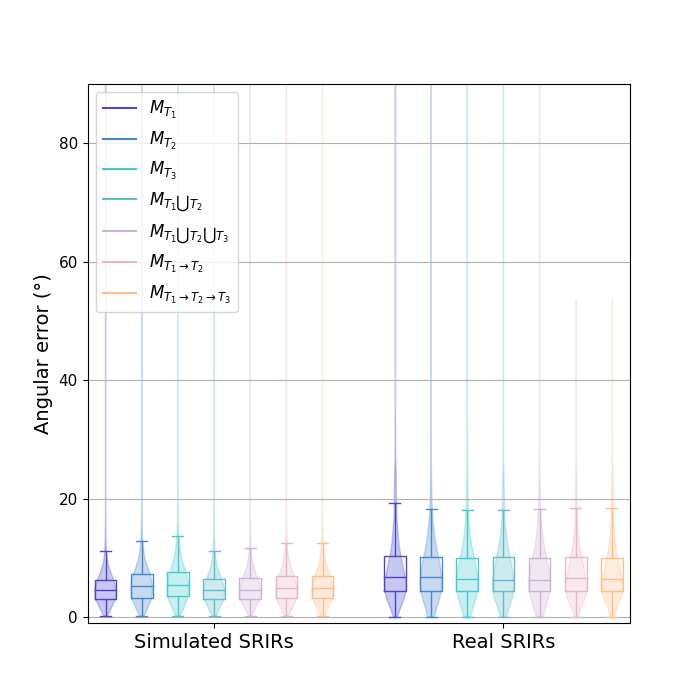
\includegraphics[width=.45\textwidth]{Images/chap7/boxplots_trainingOrder_1src.png}
    \label{subfig:multiLoca_trainingScheme_bp_1src}}
    \subfloat[2-speaker signals]{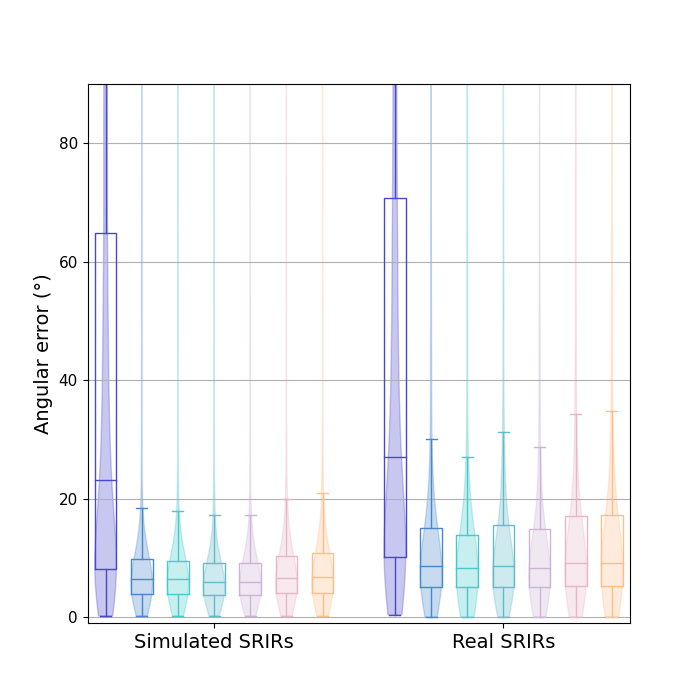
\includegraphics[width=.45\textwidth]{Images/chap7/boxplots_trainingOrder_2src.png} \label{subfig:multiLoca_trainingScheme_bp_2src}}
    \subfloat[3-speaker signals]{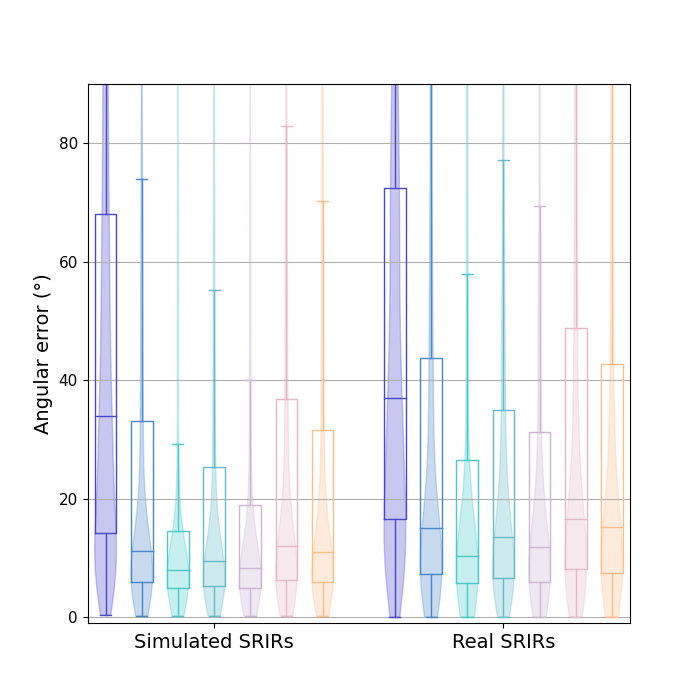
\includegraphics[width=.45\textwidth]{Images/chap7/boxplots_trainingOrder_3src.png} \label{subfig:multiLoca_trainingScheme_bp_3src}}}
    
    \captionof{figure}[Boxplots of the angular errors of the baseline CRNN for different training schemes]{Boxplots of the angular errors of the baseline CRNN for different training schemes (different colors, see the legend) and evaluated on the test datasets $E^{Sim}_1$ and $E^{Real}_1$ (left), $E^{Sim}_2$ and $E^{Real}_2$ (middle), and $E^{Sim}_3$ and $E^{Real}_3$ (right).}
    \label{fig:multiLoca_boxplots_trainingSchemes}
\end{figure}

The results are displayed in Table~\ref{tab:multiLoca_trainingSchemes} and Fig.~\ref{fig:multiLoca_boxplots_trainingSchemes}. First, we see that all models perform accurately and approximately the same on $1$-speaker signals: We obtain at least $90$\% and $98$\% accuracy on $E^{Sim}_1$ for a tolerance of $10$\textdegree~and $15$\textdegree, respectively, and more than $72$\% and $88$\% on $E^{Real}_1$. While this is not surprising for the models $M_{T_1}$, $M_{T_1 \bigcup T_2}$, $M_{T_1 \bigcup T_2 \bigcup T_3}$, $M_{T_1 \rightarrow T_2}$ and $M_{T_1 \rightarrow T_2 \rightarrow T_3}$, which are trained with $1$-speaker signals, the good accuracy obtained by models $M_{T_2}$ and $M_{T_3}$ shows that we can train the network only with $3$-speaker signals (and thus less training examples than for other models) and it will still be good at localizing $1$ or $2$ speakers. However, note that in this experiment the NoS is assumed known, so we do not take an interest in the network output variations depending on how it has been trained (\emph{e.g.}, a possible observation is that a network trained only on $3$-speakers signals may always output $3$ prominent peaks even on $2$-speaker mixtures). A last interesting observation is that $M_{T_1}$ is the best performing model on $E^{Sim}_1$, which was somewhat expected, but is the worst performing one on $E^{Real}_1$, even if the metrics are still quite high.

Next, when looking at the results on $2$-speaker signals for $E^{Sim}_2$ and $E^{Real}_2$, we immediately notice that the model $M_{T_1}$ is less accurate in localizing $2$ simultaneous speakers than the models that have been purposely trained with $2$- or $3$-speaker mixtures. For simulated SRIRs, the angular error for $M_{T_1}$ is more than $23$\textdegree~while for other models it is about $6$--$7$\textdegree. This strengthens the intuition that the network cannot perform well a task that is harder than what it encountered during training. We also observe that the models $M_{T_1 \rightarrow T_2}$ and $M_{T_1 \rightarrow T_2 \rightarrow T_3}$ are less accurate that the models $M_{T_2}$ and $M_{T_1 \bigcup T_2}$, and $M_{T_3}$ and $M_{T_1 \bigcup T_2 \bigcup T_3}$,, respectively, suggesting that fine-tuning might not be optimal for multi-speaker localization, perhaps because the pretraining on $1$-speaker signals reaches local optimum from which it becomes difficult for fine-tuning to generalize to $2$- and $3$- speaker conditions. The best performing models on $2$-speaker mixtures are those trained without fine-tuning and including $2$- or $3$-speaker signals during the training, \emph{i.e.}, models $M_{T_2}$, $M_{T_3}$, $M_{T_1 \bigcup T_2}$ and $M_{T_1 \bigcup T_2 \bigcup T_3}$.

Finally, the results on the $3$-speaker datasets confirm the analysis done in the previous paragraph. We see that the models $M_{T_1}$ and $M_{T_2}$ struggle to localize $3$ speakers as they never encounter such signals during their learning. Similarly, we remark that the fine-tuned model $M_{T_1 \rightarrow T_2 \rightarrow T_3}$ is less accurate than models $M_{T_3}$ and $M_{T_1 \bigcup T_2 \bigcup T_3}$, probably for the same reasons as explained above. On these datasets, the best performing model is $M_{T_3}$.

To sum up, these results indicate that a network trained on signals with few speakers is not able to localize many speakers, whereas, in contrast, a network trained on signals with many speakers is also able to predict the DoAs of fewer speakers. We also find out that fine-tuning is not the best option, presumably because the first training has already reached a local optimum in the network capabilities. It seems that the best option is one of the two schemes: training the network on mixtures with the highest NoS encountered in the test data, or training it with various mixtures, containing all the different considered NoS. For the remaining of this chapter, we choose the training scheme in which all the data are mixed together, as for model $M_{T_1 \bigcup T_2 \bigcup T_3}$ and as in \cite{perotin_crnn-based_2019}, except for the experiment presented in Section~\ref{ss:hoaExperiment} as we will explain later.

\subsection{Design of the feature extraction module}
\label{ss:multiLocalizationfeatureExtractionModule}

\subsubsection{Experiment objective}

\begin{figure}[t]
    \centering
    \begin{adjustbox}{width=1.\textwidth,center}
        \subfloat[Feature extraction module]{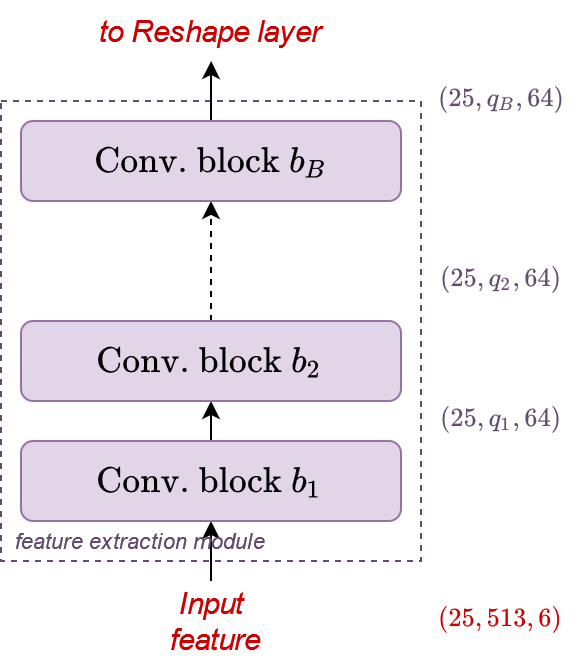
\includegraphics[width=0.45\linewidth]{Images/chap7/FeatureExtractionModule.png}
        \label{fig:multiLoca_featureExtractionModule}}
        \hspace{1cm}
        \subfloat[Convolutional block]{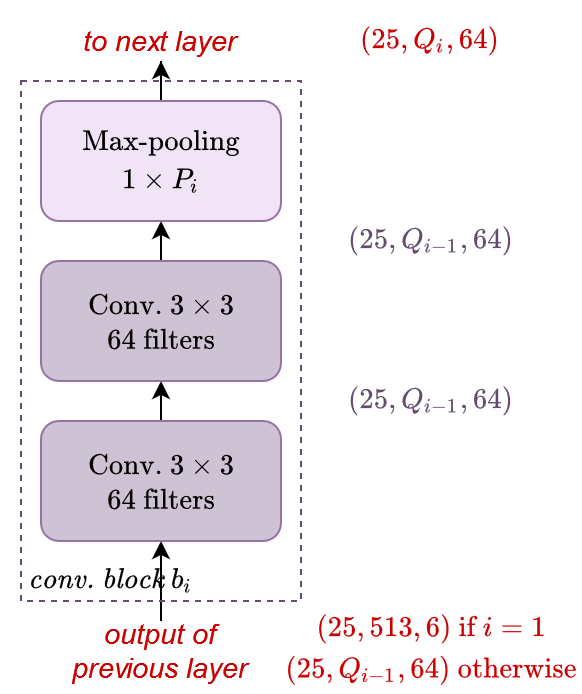
\includegraphics[width=0.35\linewidth]{Images/chap7/convolutionalBlock.png}
        \label{fig:multiLoca_featureExtractionConvolutionalBlock}}
    \end{adjustbox}
    
    \captionof{figure}[Feature extraction module and convolutional block]{Architecture of the feature extraction module and of an elementary convolutional block.}
    \label{fig:multiLoca_featureExtraction}
\end{figure}


In this experiment we focus on the design of the feature extraction module, which is directly fed with the input feature as illustrated in Fig.~\ref{fig:generalMultiLocalizationNetwork}. In \cite{perotin_crnn-based_2019}, feature extraction is done using three convolutional layers, each followed by a max-pooling layer of size $1 \times 8$, $1 \times 8$ and $1 \times 4$, respectively (see Fig.~\ref{fig:perotinCRNN}). The relatively large pooling size leads to an important loss of information between each pair of successive convolutional layers. This choice might have been guided by the necessity to reduce the second dimension before the reshape layer (possibly for the same reasons why some networks did not train properly in Chapter~\ref{chap:tdvv}). Losing such information could be detrimental for a proper feature extraction. In parallel, we believe that increasing the number of convolutional layers could help the network to find a better feature representation before the reshape layer.

For these reasons, we explore two changes to the baseline architecture: more convolutional layers and smaller pooling sizes. The newly proposed feature extraction module is illustrated in Fig.~\ref{fig:multiLoca_featureExtractionModule}. It is composed of $B$ successive convolutional blocks, where $B$ is a hyperparameter in this experiment. Each convolutional block $b_i$ consists of $2$ successive convolutional layers with $64$ filters of size $3 \times 3$ followed by a max-pooling layer of size $1 \times P_i$, where $P_i$ is another hyperparameter of this experiment and varies according to the convolutional block $b_i$. In Fig.~\ref{fig:multiLoca_featureExtractionConvolutionalBlock}, $Q_i$ denotes the second dimension of the operated tensors and is computed as $Q_i = \frac{Q_{i-1}}{P_i}$.

\begin{table}[t]
\centering
    \begin{tabular}{|c|c|c|c|c|c|c|c|c|}
        \hline
        \textbf{Model label} & \textbf{\# parameters} & \textbf{$P_1$} & \textbf{$P_2$} & \textbf{$P_3$} & \textbf{$P_4$} & \textbf{$P_5$} & \textbf{$P_6$} & \textbf{$P_7$} \\\hline
        $M_{4,2}$ & 700\,259 & 8 & 4 & 4 & 2 & - & - & - \\
        $M_{4,4}$ & 765\,795 & 4 & 4 & 4 & 2 & - & - & - \\
        $M_{4,8}$ & 896\,867 & 4 & 4 & 2 & 2 & - & - & - \\
        $M_{5,2}$ & 774\,315 & 4 & 4 & 4 & 2 & 2 & - & - \\
        $M_{5,4}$ & 839\,851 & 4 & 4 & 2 & 2 & 2 & - & - \\
        $M_{6,2}$ & 848\,371 & 4 & 4 & 2 & 2 & 2 & 2 & - \\
        $M_{6,4}$ & 913\,907 & 4 & 2 & 2 & 2 & 2 & 2 & - \\
        $M_{7,2}$ & 922\,427 & 4 & 2 & 2 & 2 & 2 & 2 & 2 \\
        $M_{7,4}$ & 987\,963 & 2 & 2 & 2 & 2 & 2 & 2 & 2 \\
        \hline
    \end{tabular}
    
    \captionof{table}[Max-pooling sizes of the successive convolutional blocks $b_i$ of the feature extraction module]{Max-pooling sizes of the successive convolutional blocks $b_i$ of the proposed feature extraction module with the number of parameters in the corresponding neural network.}
    \label{tab:featureExtractionModuleHyperparameters}
\end{table}

Whereas in \cite{perotin_crnn-based_2019} the authors used a max-pooling layer after each convolutional layer, in this new design, we use only one max-pooling layer after two successive convolutional layers in each convolutional block, so that the network has more information to extract useful features before downsampling the second dimension. In order to assess this idea, we try several combinations of hyperparameters $B$ and $P_i, i \in {1,...,B}$. The max-pooling sizes $P_i$ are chosen so that the second dimension just before the reshape layer is $2$, $4$ or $8$. Table \ref{tab:featureExtractionModuleHyperparameters} summarizes the tested configurations, along with the resulting number of parameters in the network for fair comparison. We label the models $M_{B,Q_B}$, where $B$ is the number of convolutional blocks and $Q_B$ the second dimension of the output of the last convolutional block.

\subsubsection{Results}

\begin{table}[t]
    \centering
    \subfloat[Simulated SRIRs]{
        \begin{adjustbox}{width=1.3\textwidth,center}
            \begin{tabular}{|c|cccc|cccc|cccc|}
                \hline
                \multirow{3}{*}{\textbf{Model label}} & \multicolumn{4}{c|}{\textbf{$E^{Sim}_1$}}                                                      & \multicolumn{4}{c|}{\textbf{$E^{Sim}_2$}}                                                     & \multicolumn{4}{c|}{\textbf{$E^{Sim}_3$}}                                                     \\ \cline{2-13}
                
                & \multicolumn{2}{c}{\textbf{Accuracy (\%)}} & \multicolumn{2}{c|}{\textbf{Angular error (°)}} & \multicolumn{2}{c}{\textbf{Accuracy (\%)}} & \multicolumn{2}{c|}{\textbf{Angular error (°)}}& \multicolumn{2}{c}{\textbf{Accuracy (\%)}} & \multicolumn{2}{c|}{\textbf{Angular error (°)}} \\
                
                & \textbf{\textless{}10°} & \textbf{\textless{}15°} & \textbf{Mean} & \textbf{Median} & \textbf{\textless{}10°} & \textbf{\textless{}15°} & \textbf{Mean} & \textbf{Median} & \textbf{\textless{}10°} & \textbf{\textless{}15°} & \textbf{Mean} & \textbf{Median} \\ \hline
                Baseline & 94.6                         & 99.2                         & 5.2           & 4.7           & 77.6                         & 85.7                         & 15.3          & 6.0           & 57.1                         & 68.1                         & 27.2          & 8.3           \\
                $M_{4,2}$                        & 97.6                         & 99.6                         & 4.7           & 4.2           & 86.7                         & 92.5                         & 8.3          & 4.9           & 71.4                         & 79.9                         & 15.0          & 6.3           \\
                $M_{4,4}$                        & 98.3                         & \textbf{99.7}                         & 4.5           & \textbf{4.1}           & 87.9                         & 92.7                         & 8.5          & 4.8           & 71.2                         & 79.5                         & 15.4          & 6.2           \\
                $M_{4,8}$                        & 98.2                         & 99.6                         & 4.5           & \textbf{4.1}           & 88.0                         & 92.6                         & 8.4          & 4.8           & 72.2                         & 80.7                         & 14.7          & 6.1           \\
                $M_{5,2}$                        & 98.3                         & \textbf{99.7}                         & 4.6           & \textbf{4.1}           & 87.9                         & 92.8                         & 8.0          & 4.7           & 72.5                         & 80.5                         & 14.6          & 6.1           \\
                $M_{5,4}$                        & 98.4                         & \textbf{99.7}                         & 4.6           & \textbf{4.1}           & 88.8                         & 93.1                         & 8.1          & 4.7           & 73.3                         & 81.0                         & 14.9          & 6.1           \\
                $M_{6,2}$                        & 98.4                         & 99.5                         & 4.7           & \textbf{4.1}           & 88.7                         & 93.2                         & 8.1          & 4.8           & 72.2                         & 80.7                         & 14.4          & 6.1           \\
                $M_{6,4}$                        & \textbf{98.6}                         & \textbf{99.7}                         & \textbf{4.4}           & \textbf{4.1}           & 88.3                         & 93.3                         & \textbf{7.7}          & 4.7           & \textbf{74.7}                         & \textbf{83.4}                         & \textbf{12.8}          & 5.9           \\
                $M_{7,2}$                        & 97.8                         & 99.5                         & 4.7           & \textbf{4.1}           & 86.3                         & 92.0                         & 8.6          & 4.8           & 68.6                         & 77.4                         & 16.3          & 6.5           \\
                $M_{7,4}$                        & 98.4                         & \textbf{99.7}                         & \textbf{4.4}           & \textbf{4.1}           & \textbf{89.2}                         & \textbf{93.5}                         & 7.8          & \textbf{4.6}           & 74.4                         & 81.3                         & 14.1          & \textbf{5.8}           \\ \hline
            \end{tabular}
            \label{tab:multiLoca_featureExtraction_resultsSimulatedSRIRs}
        \end{adjustbox}
    }
        
    \subfloat[Real SRIRs]{
        \begin{adjustbox}{width=1.3\textwidth,center}
            \begin{tabular}{|c|cccc|cccc|cccc|}
                \hline
                \multirow{3}{*}{\textbf{Model label}} & \multicolumn{4}{c|}{\textbf{$E^{Real}_1$}}                                                      & \multicolumn{4}{c|}{\textbf{$E^{Real}_2$}}                                                     & \multicolumn{4}{c|}{\textbf{$E^{Real}_3$}}                                                     \\ \cline{2-13}
                
                & \multicolumn{2}{c}{\textbf{Accuracy (\%)}} & \multicolumn{2}{c|}{\textbf{Angular error (°)}} & \multicolumn{2}{c}{\textbf{Accuracy (\%)}} & \multicolumn{2}{c|}{\textbf{Angular error (°)}}& \multicolumn{2}{c}{\textbf{Accuracy (\%)}} & \multicolumn{2}{c|}{\textbf{Angular error (°)}} \\
                
                & \textbf{\textless{}10°} & \textbf{\textless{}15°} & \textbf{Mean} & \textbf{Median} & \textbf{\textless{}10°} & \textbf{\textless{}15°} & \textbf{Mean} & \textbf{Median} & \textbf{\textless{}10°} & \textbf{\textless{}15°} & \textbf{Mean} & \textbf{Median} \\ \hline
                
                Baseline & 75.2                         & 91.9                         & 8.3          & 6.3           & 59.8                         & 75.2                         & 16.7          & 8.3           & 44.3                         & 58.4                         & 26.2          & 11.9          \\
                $M_{4,2}$                        & 77.7                         & 92.9                        & 8.1           & \textbf{6.1}           & 67.5                         & 83.6                         & 12.9          & 7.4           & 53.3                         & 67.5                         & 21.3          & 9.2           \\
                $M_{4,4}$                        & 77.7                         & 93.2                         & 7.9           & \textbf{6.1}           & 66.7                         & 83.4                         & 12.9          & 7.5           & 54.0                         & 69.2                         & 20.4          & 9.1           \\
                $M_{4,8}$                        & 77.8                         & 92.7                         & 8.1           & \textbf{6.1}           & 69.2                         & 84.1                         & 12.5          & 7.2           & 54.8                         & 69.7                        & 20.5          & 9.1           \\
                $M_{5,2}$                        & 77.0                         & 93.6                         & 7.9           & 6.2           & 68.1                         & 84.1                         & 12.1          & 7.3           & 55.3                         & 69.6                         & 18.7          & 8.9           \\
                $M_{5,4}$                        & 78.7                         & \textbf{93.8}                         & \textbf{7.6 }         & 6.2           & \textbf{70.2}                        & 86.0                         & 12.0          & \textbf{7.0 }         & 55.4                        & 70.9                        & 19.7          & 8.9           \\
                $M_{6,2}$                        & 78.1                         & 93.6                       & \textbf{7.6}           & \textbf{6.1}           & 68.5                         & 84.8                         & 11.9          & 7.1           & 53.9                         & 69.3                         & 19.7          & 9.1           \\
                $M_{6,4}$                        & 79.0                         & 93.7                         & \textbf{7.6}           & \textbf{6.1}           & 68.2                         & 84.7                         & 11.9          & 7.2           & 56.8                        & \textbf{73.3}                         & \textbf{17.3}          & 8.7           \\
                $M_{7,2}$                        & 76.6                         & 93.4                         & 7.7           & 6.3           & 68.0                         & 83.7                        & 12.2          & 7.2           & 53.3                         & 66.8                         & 20.9          & 9.3           \\
                $M_{7,4}$                        & \textbf{79.8}                         & 93.6                         & 7.7           & \textbf{6.1}           & 68.6                         &\textbf{86.2}                         & \textbf{11.7}          & 7.2           & \textbf{56.9}                         & 70.7                         & 19.6          & \textbf{8.6}           \\ \hline
            \end{tabular}
        \end{adjustbox}
    }
    
    \subfloat[Real recordings]{
        \begin{adjustbox}{width=1.3\textwidth,center}
            \begin{tabular}{|c|ccccc|ccccc|ccccc|ccccc|}
                \hline
                \multirow{3}{*}{\textbf{Model label}} & \multicolumn{5}{c|}{\textbf{$E^{Rec}_1$}}                                                                                                             & \multicolumn{5}{c|}{\textbf{$E^{Rec}_2$}}                                                                                                            & \multicolumn{5}{c|}{\textbf{$E^{Rec}_3$}}                                                                                                            & \multicolumn{5}{c|}{\textbf{$E^{Rec}_4$}}                                                                                                            \\ \cline{2-21}
                & \multicolumn{3}{c}{\textbf{Accuracy (\%)}}                                       & \multicolumn{2}{c|}{\textbf{Angular error (°)}} & \multicolumn{3}{c}{\textbf{Accuracy (\%)}}                                      & \multicolumn{2}{c|}{\textbf{Angular error (°)}} & \multicolumn{3}{c}{\textbf{Accuracy (\%)}}                                      & \multicolumn{2}{c|}{\textbf{Angular error (°)}} & \multicolumn{3}{c}{\textbf{Accuracy (\%)}}                                      & \multicolumn{2}{c|}{\textbf{Angular error (°)}} \\
                & \textbf{\textless{}10°} & \textbf{\textless{}15°} & \textbf{\textless{}20°} &   \textbf{Mean}    & \textbf{Median}  & \textbf{\textless{}10°} & \textbf{\textless{}15°} & \textbf{\textless{}20°} &  \textbf{Mean}    & \textbf{Median} & \textbf{\textless{}10°} & \textbf{\textless{}15°} & \textbf{\textless{}20°} &  \textbf{Mean}    & \textbf{Median}  & \textbf{\textless{}10°} & \textbf{\textless{}15°} & \textbf{\textless{}20°} &  \textbf{Mean}    & \textbf{Median}  \\ \hline
                Baseline     &35.8                    & 50.7                   & 96.6                & 13.5     & 14.9     & 30.5                   &68.2                    &  91.8                  & 13.9     & 14.1           & 29.5                  &  66.9             & 86.9           & 14.1              & 12.7                      & 30.3                   & 56.7                 & 85.6                   & 15.1     & 14.1       \\
                $M_{4,2}$       &40.0                    & 51.7                   & 99.2                   & 13.0     & 13.0     & 26.9                   & 71.7                   & 91.9                   & 14.0     & 12.9           & 36.0                  &  71.2             & 88.5           & 13.4              & 12.0     	                & 55.2                   & 73.1                 &  89.9                  &12.5      & 8.6         \\
                $M_{4,4}$       & 40.9                   & 50.6                   & 98.8                   &13.3      &13.0      & \textbf{34.5}          & 69.7                   & 91.6                   & 13.4     & 13.0           & 40.1                  &  70.0             & 88.4           & 12.4              &  11.8                     & 53.9                   & 71.0                   &  91.2                  & 12.2     & 8.4       \\
                $M_{4,8}$       & 36.4                   &51.5                    & 91.0                   &13.5      & 14.9     & 29.1                   & 73.3                   & 91.5                   & 14.0     & 13.0           & 41.3                  & 72.3              & 91.7           & 12.0              & 11.5                      & 52.2                   & 70.9                   & 90.8                   & 11.9     & 9.3       \\
                $M_{5,2}$       & 39.2                   &  49.7                  & 99.0                   & 13.5     & 16.1     & 27.0                   & 70.1                   & 93.1                   &13.6      & 13.6           & 40.2                  & 72.5              & 91.7           & 11.9              & 11.7                      & 52.0                   & 70.1                   & 91.6                   & 11.8     &9.2        \\
                $M_{5,4}$       & \textbf{46.5}          &   51.2                 & 98.4          & \textbf{12.4}     & \textbf{12.0}     & 32.8          & \textbf{73.4}          & 92.5                   & 13.4     & \textbf{12.5 } & 45.3                  & \textbf{77.7}              & 91.3           & 11.8              &  \textbf{10.8}            & 56.2                   & 73.6                  & 91.7                   & 11.7     & 8.1        \\
                $M_{6,2}$       & 35.3                   &  52.5                  & 95.8                   &13.7      & 14.5     & 22.4                   &   67.4                 & 90.4                   & 14.6     & 13.7           & 35.8                  & 71.7              & 90.9           & 13.7              & 12.1                      & 49.7                   & 68.1                   & 89.2                  & 12.7     &10.1        \\
                $M_{6,4}$       & 23.5                   &  49.4                  & 98.3                   & 14.4     &15.8      & 19.1                   & 66.5                   &92.4                    & 14.5     & 13.7           & 28.7                  & 62.6              & 88.4           & 13.7              &  13.3                     & 38.2                   & 59.8                   & 88.3                   & 13.8     & 13.6     \\
                $M_{7,2}$       &  32.9                  &  \textbf{55.5}         & 91.6                   & 16.0     & 13.0     & 23.2                   & 69.3                   &91.3                   & 14.7     & 13.6            & 35.8                  & 71.0              & 86.9           & 15.7              & 12.2                      & 48.8                   & 69.0                   & 89.3                   & 12.8     & 10.3     \\
                $M_{7,4}$       &  43.6                  &  49.4                  & \textbf{99.4 }         & 12.7     & 16.1     & 32.0                   & 71.5              & \textbf{93.8}          & \textbf{13.0}  & 13.0          & \textbf{45.6}         & 75.3     & \textbf{92.5}  & \textbf{11.3}     & \textbf{10.8}             & \textbf{58.8}          & \textbf{74.0}          & \textbf{92.0}       & \textbf{11.1}     & \textbf{7.6}  \\ \hline
            \end{tabular}
        \end{adjustbox}
    }
        
    \captionof{table}[Accuracy and angular errors of the models with the redesigned feature extraction module and the baseline]{Accuracy and angular errors of the models with the redesigned feature extraction module and the baseline. Best results are in bold.}
    \label{tab:multiLoca_featureExtraction_results}
\end{table}

\begin{figure}[t]
    \centering
    \makebox[\textwidth][c]{
    \subfloat[1-speaker signals]{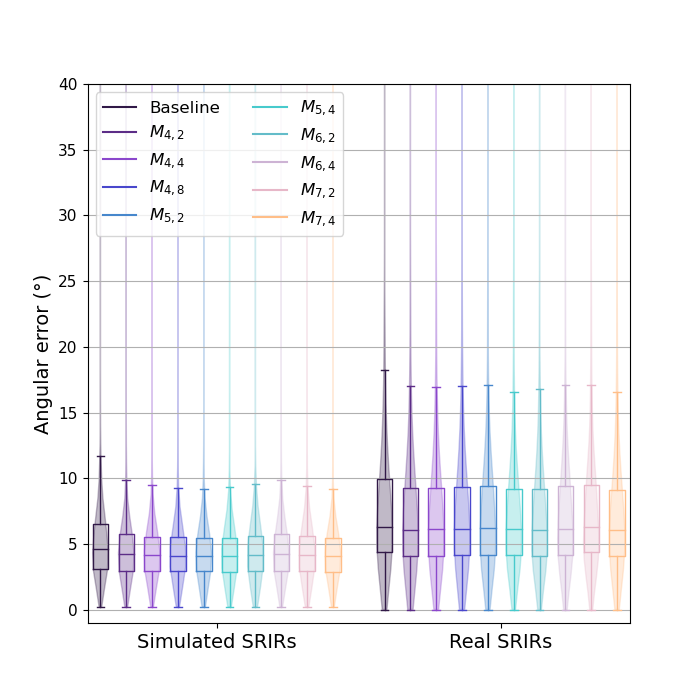
\includegraphics[width=.45\textwidth]{Images/chap7/boxplots_featureExtraction_1src.png}\label{fig:boxplots_featureExtraction_1src}}
    \subfloat[2-speaker signals]{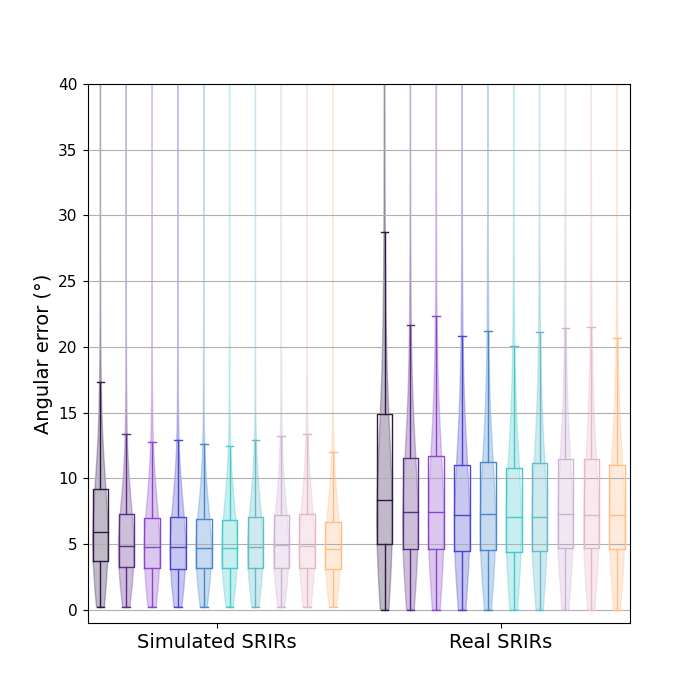
\includegraphics[width=.45\textwidth]{Images/chap7/boxplots_featureExtraction_2src.png}\label{fig:boxplots_featureExtraction_2src}}
    \subfloat[3-speaker signals]{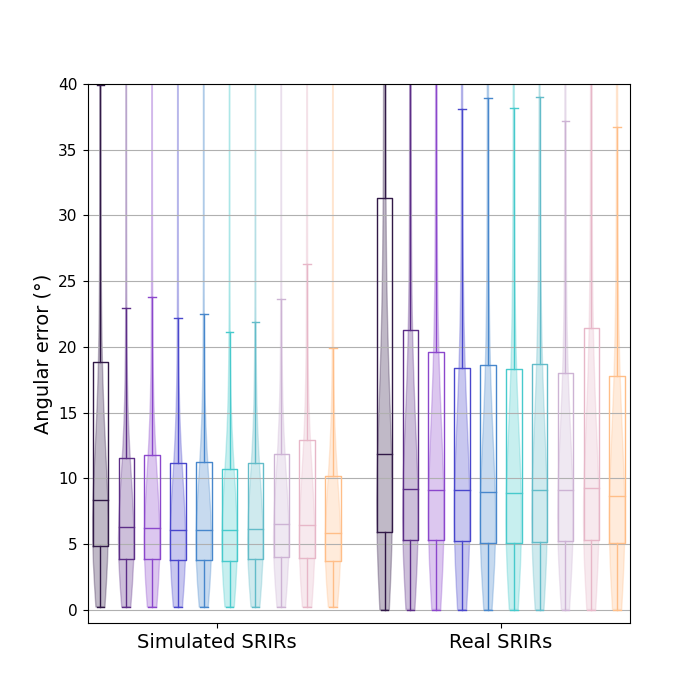
\includegraphics[width=.45\textwidth]{Images/chap7/boxplots_featureExtraction_3src.png}\label{fig:boxplots_featureExtraction_3src}}}
    
    \captionof{figure}[Boxplots of the angular errors of the models with the redesigned feature extraction module and the baseline on the simulated datasets]{Distribution of the angular errors of the models with the redesigned feature extraction module and the baseline, evaluated on the test datasets $E^{Sim}_1$ and $E^{Real}_1$ (left), $E^{Sim}_2$ and $E^{Real}_2$ (middle) and $E^{Sim}_3$ and $E^{Real}_3$ (right).}
    \label{fig:boxplots_multiLoca_featureExtraction}
\end{figure}

\begin{figure}[t]
    \centering
    \begin{adjustbox}{width=1.3\textwidth,center}
        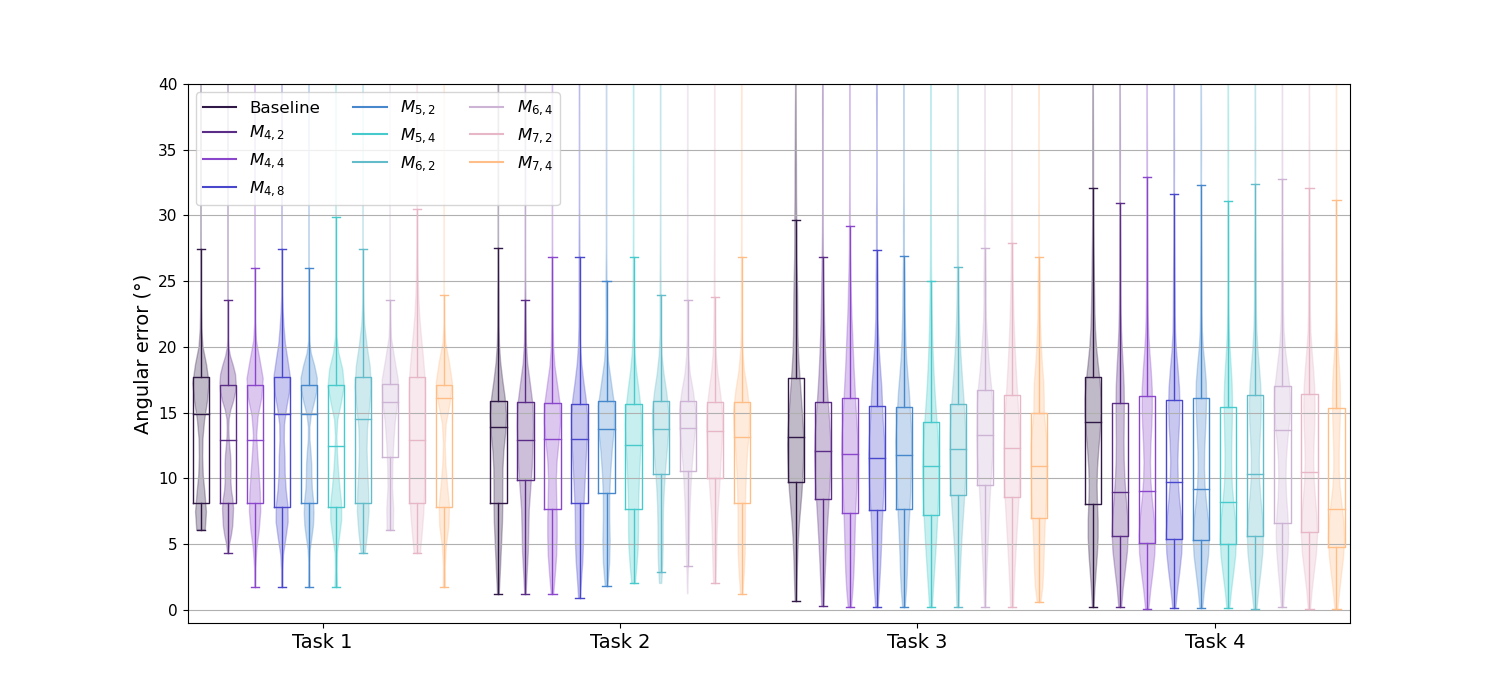
\includegraphics[width=1.\textwidth]{Images/chap7/boxplots_featureExtraction_locata.png}
    \end{adjustbox}
    
    \captionof{figure}[Boxplots of the angular errors of the models with the redesigned feature extraction module and the baseline on the recorded dataset]{Distribution of the angular errors of the models with the redesigned feature extraction module and the baseline, evaluated on the test datasets $E^{Rec}_1$ (left), $E^{Rec}_2$ (middle left), $E^{Rec}_3$ (middle right) and $E^{Rec}_4$ (right).}
    \label{fig:boxplots_multiLoca_featureExtraction_locata}
\end{figure}


Table~\ref{tab:multiLoca_featureExtraction_results} shows the results of all models on the test datasets with simulated and real SRIRs, as well as those from the various tasks of the LOCATA challenge. Fig.~\ref{fig:boxplots_multiLoca_featureExtraction} and Fig.~\ref{fig:boxplots_multiLoca_featureExtraction_locata} display the corresponding boxplots and violin plots of the angular error distributions on the simulated datasets and the LOCATA dataset, respectively.

When looking at the results in Table~\ref{tab:multiLoca_featureExtraction_results}, we see that all models surpass the baseline on the simulated datasets, and most of them lead to a better performance than the baseline on real recordings. Regarding $1$-speaker signals, the gain in performance is small compared to the baseline, for the datasets with simulated and real SRIRs. For the dataset $E^{Sim}_1$, the mean angular error for the baseline is $5.2$\textdegree~and at most $4.7$\textdegree~for our models, while for the dataset $E^{Real}_1$ it reaches $8.3$\textdegree~and at most $8.1$\textdegree, respectively. Looking at the accuracy is not very demonstrative since on simulated SRIRs the baseline already reached $99.2$\%. However, we see on the corresponding boxplots in Fig~\ref{fig:boxplots_featureExtraction_1src} that the angular errors are slightly less dispersed for our proposed models than for the baseline, which indicates that these models are less prone to large errors than the baseline. When looking at the results on the LOCATA datasets of task 1 (single static speaker), our models are not always better than the baseline, although some of them lead to a lower median. The baseline architecture thus seems quite well designed for localizing a single static source. However, regarding LOCATA task 3 signals (single moving speaker) our proposed feature extraction module leads to a significantly improved performance, with an accuracy (< $15$\textdegree) of at least $70.0$\% and a mean error smaller than $13.7$\textdegree~(except for $M_{7,2}$) for the new models compared to $66.9$\% and $14.1$\textdegree~for the baseline. This gain in performance is a bit surprising since none of these models are trained for moving speakers. These results could indicate that new models generalize better to unseen acoustic conditions than the baseline.

The results on $2$- and $3$-speaker signals clearly show that our proposed feature extraction module enables the network to be much more accurate than the baseline, in the multiple source scenario. With simulated SRIRs, the performance gain is conclusive: on $E^{Sim}_2$, the accuracy (< $15$\textdegree) goes from $85.7$\% to at least $92.0$\% and the mean angular error is reduced to at most $8.6$\textdegree, compared to $15.3$\textdegree~for the baseline. On $E^{Sim}_3$, the accuracy is increased from $68.1$\% for the baseline to at least $77.4$\% for the new models, with a mean error decrease from $27.2$\textdegree to at most $16.3$\textdegree. This improvement is slightly less notable on real SRIRs, where the gain in accuracy is between $8$ and $11$\% for $2$-speaker mixtures, and between $8$ and $15$\% for $3$-speaker mixtures. We also notice on the boxplots of Fig.~\ref{fig:boxplots_featureExtraction_2src} and \ref{fig:boxplots_featureExtraction_3src} that the error dispersion is greatly reduced, which indicates a more robust model. When looking at the results on the LOCATA datasets task 2 (multiple static speakers), the same observations as for task 1 can be made, \emph{i.e.}, the improvement is not really noticeable, and the models performance is on par with the baseline. Regarding task 4 (multiple moving speakers), the same conclusions as for task 3 can be drawn, which are that the new models seem to be slightly more efficient on these recorded signals. In particular, with regards to the $<10\%$ accuracy metric, most models outperform baseline with a margin larger than $20\%$.

Therefore, the results on all multi-speaker mixtures clearly demonstrate the superiority of the improved feature extraction over the one of the baseline architecture. While the performance gain is small for $1$-speaker signals, the improvement is substantial for $2$- and $3$-speaker mixtures and prove that this new feature extraction module is much more robust in multi-speaker environments. The results on LOCATA datasets reinforce this remark, and also exhibit that our proposal interestingly leads to a more robust localization performance for moving sources. It is noteworthy that the tasks 3 and 4 of the LOCATA challenge involve human talkers, as opposed to tasks 1 and 2 where loudspeakers are used as sound sources. The latter are less accurately represented by point sources, which is the type of sources the networks are trained on. As intuited, using more convolutional layers and less drastic max-pooling provides more flexibility to the neural network, while it does not increase the number of parameters more than twice that of the baseline.

Now, when we compare the new models with each other, there is a little tendency that the use of deeper architectures (more convolutional layers) leads to better performance (the highest metrics are most often obtained with the model $M_{7,4}$). However, more investigation is needed to support this claim, since the observed results are insufficient to draw a firm conclusion on this aspect. Furthermore, when comparing models with the same number of convolutional blocks $B$, we notice that the best results are obtained by those with $Q_B = 4$, emphasizing the fact that downsampling information degrades the performance, although it allows a smaller number of parameters.

\clearpage
\subsection{Self-attention mechanism}
\label{ss:multiLocalizationSelfAttention}

\subsubsection{Experiment objective}

In the previous experiment, we managed to greatly improve the capability of the CRNN to localize multiple speakers in a multi-channel mixture based on the redesign of the feature extraction module. Now, we focus on the temporal analysis module, which is fed with the reshaped extracted feature as illustrated in Fig.~\ref{fig:generalMultiLocalizationNetwork}. In most neural network architectures proposed in the neural-based SSL literature, and particularly in \cite{perotin_crnn-based_2019}, such a temporal analysis module generally relies on recurrent layers, generally implemented with LSTM or GRU units (see Section~\ref{ss:recurrentNeuralNetworks}). The advantage of such layers is their capacity of processing relatively long sequences and in the case of SSL, they can potentially learn the evolution of a speech sentence characteristics in order to improve the localization performance. However, this comes with the limitation of processing the temporal dimension in a sequential way, while some crucial information for localization likely lie in specific and isolated frames anywhere in the sequence, \emph{e.g.}, frames with transients as pointed out in \cite{perotin_localisation_2019}. Another limitation of such recurrent layers, due to their processing following a temporal order, is that it is not possible to parallelize the computation of the output sequence. This computational cost can be an important constraint towards real-time devices.

We therefore propose to replace the BiLSTM layers, as used in the previous experiments and the baseline, with multi-head self-attention encoders introduced in \cite{vaswani_attention_2017}. In this new experiment, we employ the feature extraction module of the model $M_{6,4}$ \footnote{Although Section~\ref{ss:multiLocalizationfeatureExtractionModule} showed that this model does not give the best results, we chose to base the current study on this model at a time when we did not collected all the evaluation data.}. Therefore, the model $M_{6,4}$, which includes recurrent layers (as do all models discussed in the previous sections), is the baseline in this new experiment. As illustrated in Fig.~\ref{fig:multiLoca_TemporalAnalysisModule}, the temporal analysis module contains $E$ Transformer encoders, as represented in Fig.~\ref{fig:transformerEncoder}, where $E$ is an hyperparameter in this experiment. In each encoder, we either employ multi-head or cross-multi-head self-attention, with $H$ heads, $H$ being another hyperparameter.

\begin{figure}[t]
    \centering
    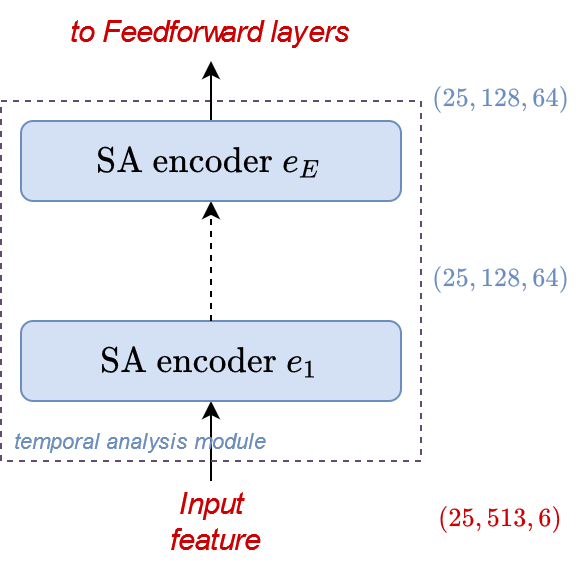
\includegraphics[width=0.45\linewidth]{Images/chap7/TemporalAnalysisModule.png}
    \captionof{figure}[Temporal analysis module with self-attention encoders]{Architecture of the temporal analysis module of the proposed CNN including a series of self-attention encoders.}
    \label{fig:multiLoca_TemporalAnalysisModule}
\end{figure}

Table~\ref{tab:selfAttentionHyperparameters} details the different values of hyperparameters we try in this experiment. We first evaluate the benefit of using classical multi-head self-attention using $1$ encoder and $H$ heads, with $H \in \{1, 2, 3, 10\}$. These models are labelled $\text{MH-} 1\text{enc-} H\text{H}$. Then, we compare the use of cross-multi-head self-attention over multi-head self-attention for $1$ encoder with $H = 3$ or $10$ heads. Finally we assess the addition of another encoder ($E=2$), first with $H=10$ to directly compare with $E=1$, and also with $H=5$ to compare the performance of $2$ encoders with $5$ heads against $1$ encoder with $10$ heads.

\begin{table}[t]
\centering
\begin{tabular}{|c|c|c|c|c|}
\hline
\textbf{Model label}                    & \textbf{\# parameters} & \textbf{SA type} & \textbf{$E$} & \textbf{$H$} \\ \hline
$M_{\text{MH-}1\text{enc-}1\text{H}}$   & 796\,125               & MH               & 1            & 1            \\
$M_{\text{MH-}1\text{enc-}2\text{H}}$   & 862\,045               & MH               & 1            & 2            \\
$M_{\text{MH-}1\text{enc-}3\text{H}}$   & 927\,965               & MH               & 1            & 3            \\
$M_{\text{MH-}1\text{enc-}10\text{H}}$  & 1\,389\,405            & MH               & 1            & 10           \\
$M_{\text{CMH-}1\text{enc-}3\text{H}}$  & 927\,965               & CMH              & 1            & 3            \\
$M_{\text{CMH-}1\text{enc-}10\text{H}}$ & 1\,389\,405            & CMH              & 1            & 10           \\
$M_{\text{CMH-}2\text{enc-}5\text{H}}$  & 1\,653\,341            & CMH              & 2            & 5            \\
$M_{\text{CMH-}2\text{enc-}10\text{H}}$ & 2\,312\,541            & CMH              & 2            & 10    \\ \hline      
\end{tabular}
\captionof{table}[Values of hyperparameters experimented in the temporal analysis module using self-attention]{Values of hyperparameters experimented in each encoder of the temporal analysis module using self-attention.}
    \label{tab:selfAttentionHyperparameters}
\end{table}

\subsubsection{Results}

\begin{table}[t]
    \centering
    
    \subfloat[Simulated SRIRs]{
        \begin{adjustbox}{width=1.3\textwidth,center}
            \begin{tabular}{|c|cccc|cccc|cccc|}
            \hline
            \multirow{2}{*}{\textbf{Model}} & \multicolumn{4}{c|}{\textbf{1 source}}                                                      & \multicolumn{4}{c|}{\textbf{2 sources}}                                                     & \multicolumn{4}{c|}{\textbf{3 sources}}                                                     \\
                                            & \textbf{Acc. \textless{}10°} & \textbf{Acc. \textless{}15°} & \textbf{Mean} & \textbf{Med.}  & \textbf{Acc. \textless{}10°} & \textbf{Acc. \textless{}15°} & \textbf{Mean} & \textbf{Med.}  &\textbf{Acc. \textless{}10°} & \textbf{Acc. \textless{}15°} & \textbf{Mean} & \textbf{Med.}  \\ \hline
            Baseline ($M_{6,4}$)                 & \textbf{98.6}                         & 99.7                         & \textbf{4.4}           & \textbf{4.1}           & 88.3                         & 93.3                         & 7.7           & \textbf{4.7}            & 74.7                         & 83.4                        & 12.8          & 5.9          \\
            $M_{\text{MH-}1\text{enc-}1\text{H}}$                     & 98.3                         & 99.7                         & 4.5           & 4.2            & 87.9                         & 93.6                         & 7.9           & 4.9          & 71.6                         & 81.5                         & 13.5          & 6.5           \\
            $M_{\text{MH-}1\text{enc-}2\text{H}}$                      & 98.1                         & 99.7                         & 4.7           & 4.2          & 87.1                         & 93.0                         & 8.7           & 4.9     & 72.2                         & 80.6                         & 15.8          & 6.2         \\
            $M_{\text{MH-}1\text{enc-}3\text{H}}$                      & 98.1                         & 99.6                         & 4.7           & 4.2          & 87.7                         & 92.7                         & 8.8           & 4.8      & 72.9                         & 80.7                         & 16.2          & 6.0         \\
            $M_{\text{MH-}1\text{enc-}10\text{H}}$                     & 98.5                         & 99.6                         & 4.5           & \textbf{4.1}          & \textbf{90.4}                         & 94.5                         & 7.4           & \textbf{4.7}          & 77.3                         & 84.7                         & 12.3          & \textbf{5.6}         \\
            $M_{\text{CMH-}1\text{enc-}3\text{H}}$                      & 98.5                         & \textbf{99.8}                         & \textbf{4.4}           & \textbf{4.1}         & 89.3                         & 94.1                         & 7.6           & 4.8        & 75.9                         & 84.1                         & 12.7          & 5.9        \\
            $M_{\text{CMH-}1\text{enc-}10\text{H}}$                     & 98.4                         & 99.5                         & 4.5           & \textbf{4.1}           & 89.9                         & 94.5                         & \textbf{6.8}           & \textbf{4.7}        & \textbf{78.2}                         & \textbf{85.7}                         & \textbf{11.3}          & \textbf{5.6}         \\
            $M_{\text{CMH-}2\text{enc-}5\text{H}}$                      & 98.5                         & 99.6                         & 4.6           & 4.2          & \textbf{90.4}                         & 94.7                         & 7.0           & \textbf{4.7}           & 75.6                         & 84.2                         & 12.4          & 6.0         \\
            $M_{\text{CMH-}2\text{enc-}10\text{H}}$                    & 97.9                         & 99.3                         & 4.8           & 4.2        & 88.7                         & \textbf{94.9}                         & 7.3           & 5.0          & 72.8                         & 83.7                         & 13.0          & 6.5          \\ \hline
            \end{tabular}
        \end{adjustbox}
    }

    \subfloat[Real SRIRs]{
    \begin{adjustbox}{width=1.3\textwidth,center}
        \begin{tabular}{|c|cccc|cccc|cccc|}
        \hline
        \multirow{2}{*}{\textbf{Model}} & \multicolumn{4}{c|}{\textbf{1 source}}                                                      & \multicolumn{4}{c|}{\textbf{2 sources}}                                                     & \multicolumn{4}{c|}{\textbf{3 sources}}                                                     \\
                                        & \textbf{Acc. \textless{}10°} & \textbf{Acc. \textless{}15°} & \textbf{Mean} & \textbf{Med.} & \textbf{Acc. \textless{}10°} & \textbf{Acc. \textless{}15°} & \textbf{Mean} & \textbf{Med.} & \textbf{Acc. \textless{}10°} & \textbf{Acc. \textless{}15°} & \textbf{Mean} & \textbf{Med.} \\ \hline
        Baseline ($M_{6,4}$)                 & \textbf{79.0}                         & \textbf{93.7}                         & 7.6           & \textbf{6.1}          & 68.2                         & 84.7                         & 11.9          & \textbf{7.2}           & 56.8                         & 73.3                         & 17.3          & 8.7          \\
        $M_{\text{MH-}1\text{enc-}1\text{H}}$                     & 77.0                         & 93.5                         & \textbf{7.5}           & 6.2          & 67.4                         & 83.5                         & 11.5          & \textbf{7.2}           & 53.8                         & 69.9                         & 18.9          & 9.1           \\
        $M_{\text{MH-}1\text{enc-}2\text{H}}$                      & 76.8                         & 93.4                         & 7.6           & 6.3          & 67.9                         & 83.8                         & 12.7          & 7.5          & 53.6                         & 68.5                         & 22.5          & 9.1          \\
        $M_{\text{MH-}1\text{enc-}3\text{H}}$                      & 76.2                         & 92.7                         & 8.1           & 6.3          & 67.4                         & 84.9                         & 12.3          & 7.3          & 54.6                         & 68.3                         & 21.8          & 9.1          \\
        $M_{\text{MH-}1\text{enc-}10\text{H}}$                     & 77.3                         & 93.0                         & 8.3           & 6.2         & 68.2                         & 86.3                         & 11.2          & 7.3           & 57.8                         & 74.0                         & 16.9          & \textbf{8.5}          \\
        $M_{\text{CMH-}1\text{enc-}3\text{H}}$                      & 77.5                         & 92.6                         & 8.0           & 6.3         & 68.6                         & 85.6                         & 10.7          & 7.3          & 56.4                         & 72.3                         & 18.2          & 8.9           \\
        $M_{\text{CMH-}1\text{enc-}10\text{H}}$                     & 77.0                         & 92.6                         & 8.0           & 6.2          & 68.6                         & 85.8                         & 10.5          & 7.3          & \textbf{58.2}                         & \textbf{74.8}                         & \textbf{15.2}          & \textbf{8.5}         \\
        $M_{\text{CMH-}2\text{enc-}5\text{H}}$                      & 75.7                         & 92.6                         & 8.4           & 6.3          & \textbf{70.0}                         & \textbf{87.1}                         & \textbf{10.4}          & \textbf{7.2}         & 57.7                         & 74.2                         & 16.3          & 8.6          \\
        $M_{\text{CMH-}2\text{enc-}10\text{H}}$                     & 75.7                         & 91.1                         & 8.8           & 6.2          & 69.0                         & 86.9                         & 10.6          & \textbf{7.2}           & 56.3                         & 73.3                         & 17.1          & 8.9          \\ \hline
        \end{tabular}
    \end{adjustbox}
    }

    \subfloat[Real recordings]{
        \begin{adjustbox}{width=1.3\textwidth,center}
            \begin{tabular}{|c|ccccc|ccccc|ccccc|ccccc|}
                \hline
                \multirow{3}{*}{\textbf{Model label}} & \multicolumn{5}{c|}{\textbf{$E^{Rec}_1$}}                                                                                                             & \multicolumn{5}{c|}{\textbf{$E^{Rec}_2$}}                                                                                                            & \multicolumn{5}{c|}{\textbf{$E^{Rec}_3$}}                                                                                                            & \multicolumn{5}{c|}{\textbf{$E^{Rec}_4$}}                                                                                                            \\ \cline{2-21}
                & \multicolumn{3}{c}{\textbf{Accuracy (\%)}}                                       & \multicolumn{2}{c|}{\textbf{Angular error (°)}} & \multicolumn{3}{c}{\textbf{Accuracy (\%)}}                                      & \multicolumn{2}{c|}{\textbf{Angular error (°)}} & \multicolumn{3}{c}{\textbf{Accuracy (\%)}}                                      & \multicolumn{2}{c|}{\textbf{Angular error (°)}} & \multicolumn{3}{c}{\textbf{Accuracy (\%)}}                                      & \multicolumn{2}{c|}{\textbf{Angular error (°)}} \\
                & \textbf{\textless{}10°} & \textbf{\textless{}15°} & \textbf{\textless{}20°} &   \textbf{Mean}    & \textbf{Median}  & \textbf{\textless{}10°} & \textbf{\textless{}15°} & \textbf{\textless{}20°} &  \textbf{Mean}    & \textbf{Median} & \textbf{\textless{}10°} & \textbf{\textless{}15°} & \textbf{\textless{}20°} &  \textbf{Mean}    & \textbf{Median}  & \textbf{\textless{}10°} & \textbf{\textless{}15°} & \textbf{\textless{}20°} &  \textbf{Mean}    & \textbf{Median}  \\ \hline
                Baseline ($M_{6,4}$)    &35.8                    & 50.7                   & 96.6                & 13.5     & 14.9     & \textbf{30.5}                   &68.2                    &  \textbf{91.8}                  & 13.9     & 14.1           & 29.5                  &  66.9             & 86.9           & 14.1              & 12.7                      & 30.3                   & 56.7                 & 85.6                   & 15.1     & 14.1       \\
                $M_{\text{MH-}1\text{enc-}1\text{H}}$       &29.3                    & 55.4                   & 96.2                   & 13.4     & 14.5     & 27.3                   & 69.9                   & 88.4                   & \textbf{13.7}     & \textbf{12.9}           & 42.5                  &  73.2             & 90.6           & 12.5              & 11.3     	                & 41.7                   & 64.7                 &  87.7                  &13.8      & 12.3         \\
                $M_{\text{MH-}1\text{enc-}2\text{H}}$       & 33.6                   & 49.3                   & 98.9                  &13.2      &13.7      & 22.2          & 59.6                   & 77.1                   & 14.2     & 13.0           & 39.8                  &  70.6             & \textbf{91.4}           &\textbf{ 12.1}              &  11.7                     & 46.6                   & 64.2                   &  85.2                  & 12.4     & 10.2       \\
                $M_{\text{MH-}1\text{enc-}3\text{H}}$       & 29.5                   &\textbf{57.7}                   & 98.9                  &13.2      & 13.7     & 19.0                   & 59.2                   & 80.2                   & 14.6     & 13.7           & 34.5                  & 69.4              & 90.6           & 13.0              & 12.3                      & 48.8                   & \textbf{67.0}                   & 87.6                   & \textbf{11.7}     & 9.7       \\
                $M_{\text{MH-}1\text{enc-}10\text{H}}$       & 37.3                   &  50.1                  & \textbf{99.5}                   & \textbf{12.9}     & \textbf{11.9}     & 23.4                   & 66.1                   &88.0                   &14.5      & 13.6           & \textbf{44.9}                  & \textbf{75.9}              & 90.9           & 12.3             & \textbf{10.9}                      & \textbf{50.9}                   & 66.7                   & 88.2                   & 12.8     &\textbf{9.6}        \\
                $M_{\text{CMH-}1\text{enc-}3\text{H}}$      & \textbf{41.7}          &  51.1                 & 92.9          & 13.0     & 14.9     & 21.3          & 64.6 & 86.7                   & 14.6     & 13.8 & 38.9                  & 67.4              & 88.0           & 12.5              &  12.2           & 48.1                   & 66.3                  & 88.8                   &12.9     & 10.6        \\
                $M_{\text{CMH-}1\text{enc-}10\text{H}}$      & 35.2                   &  49.4                  & 98.1                   &13.5      & 16.1     & 25.3                   &   66.8                 & 87.7                   & 13.9     & \textbf{12.9}           & 42.2                  & 72.8              & 89.9           & 12.3              & 11.3                      & 48.5                   & 65.6                   & 87.3                  & 13.8     &10.4        \\
                $M_{\text{CMH-}2\text{enc-}5\text{H}}$       &35.2                   &  49.2                  & 99.3                   & 13.4     &16.1      & 25.2                   & \textbf{70.3}                   &87.6                    & 15.4     & 13.0           & 35.2                  & 63.4              & 86.9           & 13.7              &  12.5                     & 49.6                   & 66.3                   & 87.9                   & 14.0     & 10.4     \\
                $M_{\text{CMH-}2\text{enc-}10\text{H}}$      &  39.8                  &  54.6         & 98.0                   & 13.5     & 14.2     & 25.7                   & 68.7                   &88.0                   & 14.5     & 13.6            & 27.2                  & 62.9              & 86.9           & 14.7              & 13.4                      & 39.6                  & 64.6                  & \textbf{90.6}                  &14.3     & 13.4     \\ \hline
            \end{tabular}
        \end{adjustbox}
    }
        
    \captionof{table}[Accuracy and angular errors of the models with the temporal analysis module based on self-attention and the baseline]{Accuracy and angular errors of the models with the temporal analysis module based on self-attention and the baseline. Best results are in bold.}
    \label{tab:multiLoca_selfAttention_results}
\end{table}

\begin{figure}[t]
    \centering
    \makebox[\textwidth][c]{
    \subfloat[1-speaker signals]{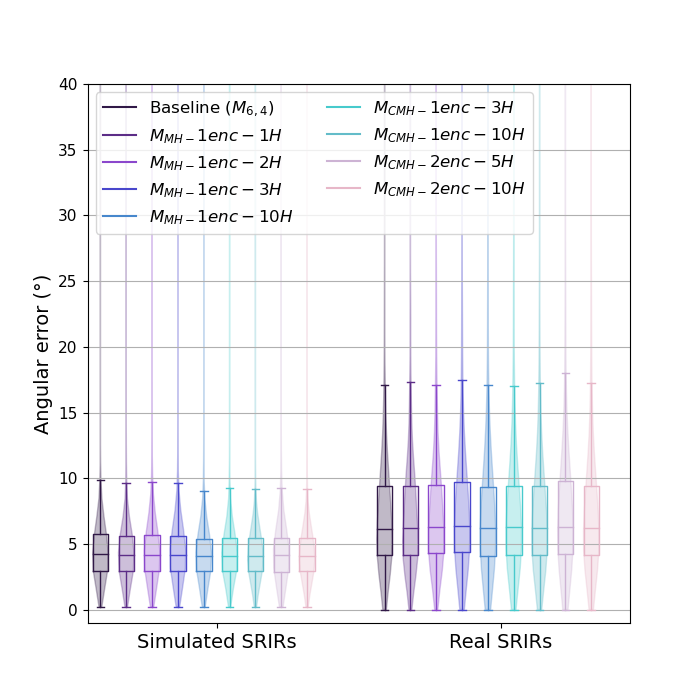
\includegraphics[width=.45\textwidth]{Images/chap7/boxplots_selfAttention_1src.png}\label{fig:boxplots_selfAttention_1src}}
    \subfloat[2-speaker signals]{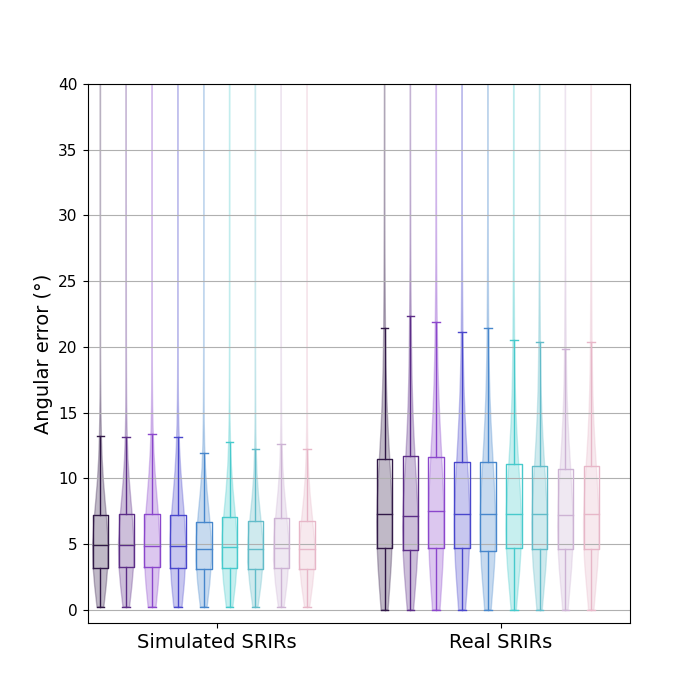
\includegraphics[width=.45\textwidth]{Images/chap7/boxplots_selfAttention_2src.png}\label{fig:boxplots_selfAttention_2src}}
    \subfloat[3-speaker signals]{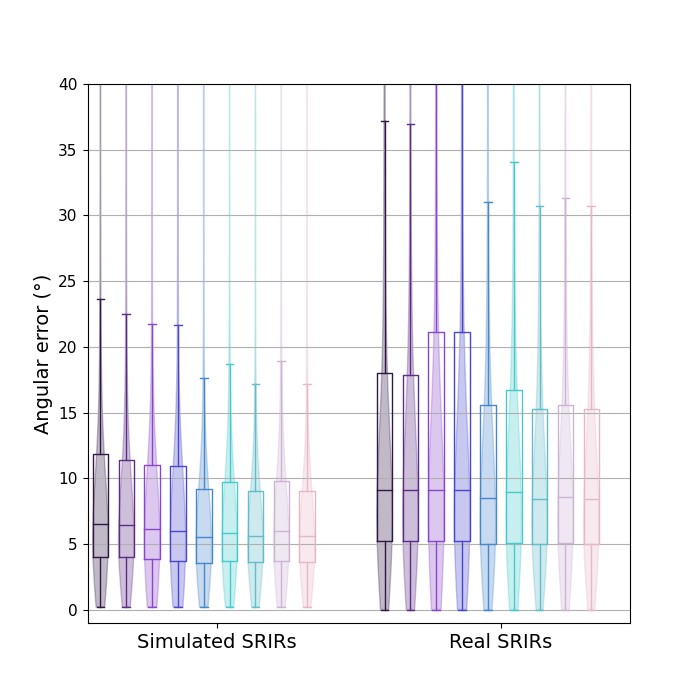
\includegraphics[width=.45\textwidth]{Images/chap7/boxplots_selfAttention_3src.png}\label{fig:boxplots_selfAttention_3src}}}
    
    \captionof{figure}[Boxplots of the angular errors of the models with the temporal analysis module based on self-attention and the baseline on the simulated datasets]{Distribution of the angular errors of the models with the temporal analysis module based on self-attention and the baseline, evaluated on the test datasets $E^{Sim}_1$, $E^{Sim}_2$, $E^{Sim}_3$, $E^{Real}_1$, $E^{Real}_2$ and $E^{Real}_3$.}
    \label{fig:boxplots_multiLoca_selfAttention}
\end{figure}

\begin{figure}[t]
    \centering
    \begin{adjustbox}{width=1.3\textwidth,center}
        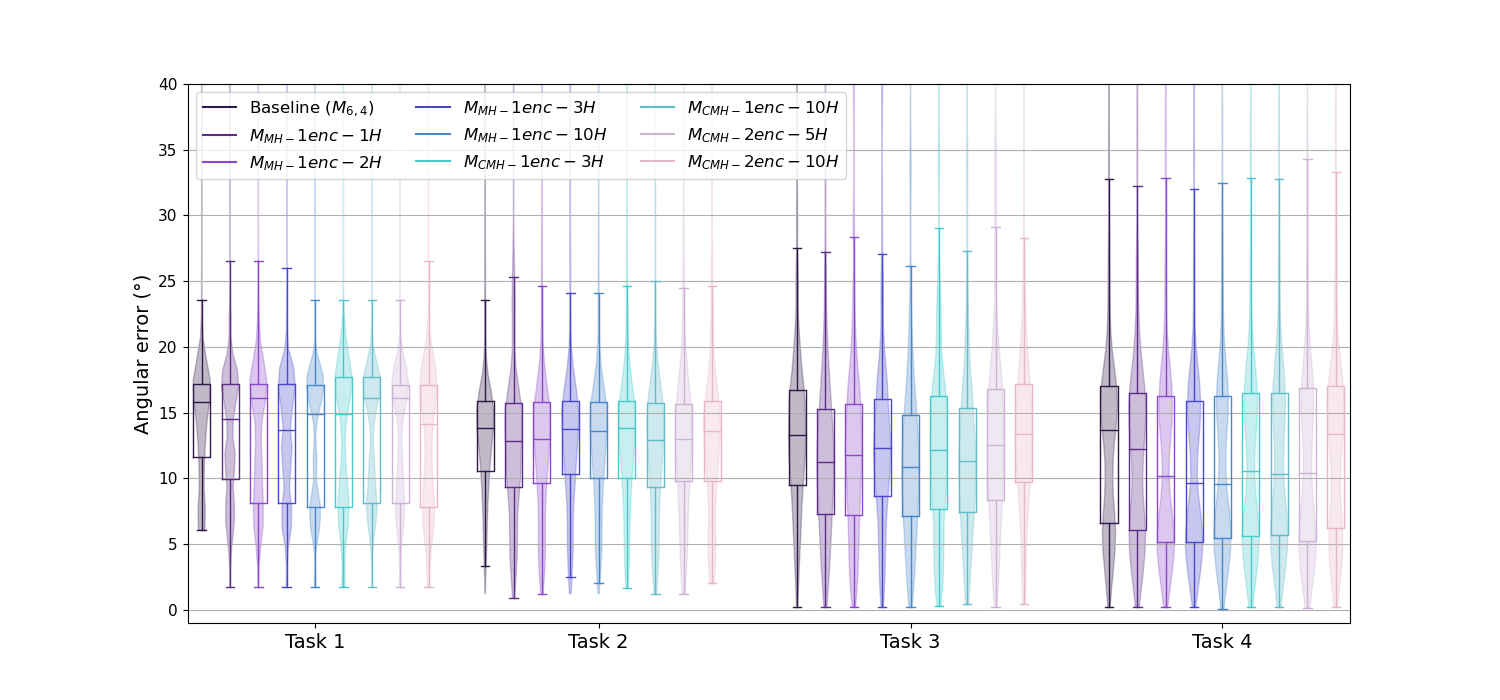
\includegraphics[width=1.\textwidth]{Images/chap7/boxplots_selfAttention_locata.png}
    \end{adjustbox}
    
    \captionof{figure}[Boxplots of the angular errors of the models with the temporal analysis module based on self-attention and the baseline on the recorded dataset]{Distribution of the angular errors of the models with the temporal analysis module based on self-attention and the baseline, evaluated on the test datasets $E^{Rec}_1$, $E^{Rec}_2$, $E^{Rec}_3$ and $E^{Rec}_4$.}
    \label{fig:boxplots_multiLoca_selfAttention_locata}
\end{figure}

The results of this experiment are reported in Table~\ref{tab:multiLoca_selfAttention_results} and Figures ~\ref{fig:boxplots_multiLoca_selfAttention} and \ref{fig:boxplots_multiLoca_selfAttention_locata}. 

First, we can see that the performance of the self-attention-based neural networks are on par with the CRNN performance, either on simulated data or real recordings. This shows that it is possible to replace the BiLSTM layers with self-attention encoders without losing in performance. Some models leads to a slightly lower performance, while others outperform the baseline. On real recordings, the improvement over the baseline is quite significant, which can be clearly observed in the boxplots in Fig.~\ref{fig:boxplots_multiLoca_selfAttention_locata}. We see that the use of self-attention encoders globally reduces the median angular error, but slightly increase the variance. Moreover, Table~\ref{tab:multiLoca_inferenceTimes} shows that the inference time of all self-attention-based models is significantly lower than the CRNN baseline, \emph{i.e.}, $44$\% lower in real-time percentage when using $1$ encoder (and $33$\% lower when using 2 encoders). This inference time does not seem to be correlated to the number of parameters but rather to the number of encoders. This was expected, since such an architecture leads to the processing of each encoder one after another. In contrast, increasing the number of heads does not increase the inference time since the matrix operations can be done in parallel in the graphical processing units (GPU) that we use in our experiments.

Second, when assessing the use of different number of heads $H$ with classical MH self-attention, we see that using self-attention with $H=1,2,3$ heads gives performance that is slightly lower than the baseline. However, the model $M_{\text{MH-}1\text{enc-}10\text{H}}$, with $H=10$ heads, is more accurate than the baseline. This improvement is also more pronounced when there are many speakers in the analyzed signal. For instance, on $3$-speaker mixtures with synthetic SRIRs, the accuracy (< $10$\textdegree) for this model is $77.3$\% while it is $74.7$\% for the baseline. Increasing the number of self-attention heads may thus be beneficial for multi-source localization. We postulate that this is due to multiple ``views'' of the same input sequence, \emph{i.e.}, the diversity provided by multiple self-attention heads.

Next, when we compare the performance for multi-head against cross-multi-head self-attention, we see that CMH leads to better results than MH, and even better results than the baseline. For example, the mean average error on $3$-speaker signals with simulated SRIRs is lowered by $3.5$\textdegree~when using CMH with $H=3$ heads, and by $1.0$\textdegree~with $H=10$. The same gain in performance can be observed on mixtures generated with real SRIRs: on $2$-speaker signals, the CMH-based model with $10$ heads leads to a mean average error of $10.5$\textdegree~vs. $11.2$\textdegree~for the MH-based model, whereas for $3$-speaker mixtures it is lower by $1.7$\textdegree. Regarding real recordings, the superiority of CMH over MH is less visible, especially because the model $M_{\text{MH-}1\text{enc-}10\text{H}}$ is one of the best performing models on real data.

Furthermore, the results when adding another self-attention encoder to the temporal analysis module are less conclusive. Model $M_{\text{CMH-}2\text{enc-}5\text{H}}$, which uses $5$ heads, is better than Model $M_{\text{CMH-}2\text{enc-}10\text{H}}$ with $10$ heads for $2$-speaker mixtures, but it loses performance for $3$-speaker mixtures. Also the first one shows a better performance on real recordings with mobile sources but has worse results when the sources are static. When comparing the use of $1$ and $2$ encoders with $H=10$ heads, the results are slightly lower for Model $M_{\text{CMH-}2\text{enc-}10\text{H}}$. This shows that stacking more encoders does not necessarily improve the performance. However, we believe that further experiments are needed for a more convincing conclusion.

\begin{table}[t]
    \centering
    \begin{tabular}{|c|cc|}
    \hline
    \textbf{Model}  & \textbf{real-time \%} & \textbf{\# parameters} \\ \hline
    Baseline ($M_{6,4}$) & 437  & 913,907    \\
    $M_{\text{MH-}1\text{enc-}1\text{H}}$      & 244  & 796,125    \\
    $M_{\text{MH-}1\text{enc-}2\text{H}}$      & 244  & 862,045    \\
    $M_{\text{MH-}1\text{enc-}3\text{H}}$      & 244  & 927,965    \\
    $M_{\text{MH-}1\text{enc-}10\text{H}}$     & 244  & 1,389,405  \\
    $M_{\text{CMH-}1\text{enc-}3\text{H}}$      & 244  & 927,965    \\
    $M_{\text{CMH-}1\text{enc-}10\text{H}}$     & 244  & 1,389,405  \\
    $M_{\text{CMH-}2\text{enc-}5\text{H}}$      & 281  & 1,653,341  \\
    $M_{\text{CMH-}2\text{enc-}10\text{H}}$     & 281  & 2,312,541  \\ \hline
    \end{tabular}
    \captionof{table}[Inference time of self-attention-based models and the baseline]{Real-time percentage for inference and number of parameters for the different tested models (in our experiments, frame length = 0.032~s).}
    \label{tab:multiLoca_inferenceTimes}
\end{table}

To conclude this experiment, we show that it is possible to replace BiLSTM layers with self-attention encoders without losing in performance, which can greatly decrease the network inference time. We see that using more attention heads seems to increase the localization accuracy, but stacking encoders does not necessarily have the same effect. However, we manage to improve the overall performance using cross-multi-head self-attention, which is especially pronounced in a multi-speaker context.

\subsection{HO-PIV \emph{v.s.} FO-PIV}
\label{ss:hoaExperiment}

\subsubsection{Experiment objective}

In this last experiment, we propose to evaluate the use of higher-order Ambisonics for the input signal. With higher Ambisonics orders, the spatial resolution is increased and therefore it provides a suitable representation, especially when the sources are spatially close to each other \cite{zotter_ambisonics_2019}. With this property, one can expect to improve the overall localization performance. For that matter, we use the extension of the normalized pseudointensity vector to the higher-order Ambisonics, namely the HO-PIV $\mathbf{\bar{I}}^N$, as presented in Section~\ref{ss:pseudointensityVector}. For practical reasons, this experiment is more limited than the previous ones in terms of data. First, we only assess the use of HO-PIV at order $N=2$, \emph{i.e.}, with $9$ Ambisonics channels, leading to input tensors of shape $25 \times 513 \times 16$ since we still stack the real and imaginary parts in the third dimension. Also, we limit the training data to $T_3$ only (\emph{i.e.}, we work with $3$-speaker mixtures) since this proved to be also quite robust on $1$- and $2$-speaker signals.\footnote{To give some insights, each dataset $T_n$ with FO-PIV is about $80$~GB big, resulting in a total of $240$~GB of training data. Such data quantity reaches $240 \times \frac{16}{6} = 640$~GB at order $2$ and $240 \times \frac{30}{6} = 1\,200$~GB at order $3$. The time necessary to process such an amount of data is prohibitively long. Since we do not want to decrease the number of room configurations in the training dataset, we limit the training to the dataset $T_3$ with HO-PIV at order $2$.}

As previously, we use odel $M_{6,4}$ trained with FO-PIV input feature as the baseline in this experiment. We then train the exact same neural network with HO-PIV input features as described above, leading to a model labelled $M^{HO}_{6,4}$. As we showed in the first experiment that limiting the training on $3$-speaker signals still gives satisfying results on $1$- and $2$-speaker mixtures, we evaluate this model on all testing datasets.

\subsubsection{Results}

\begin{table}[t]
\centering
    \subfloat[Simulated SRIRs]{
        \begin{adjustbox}{width=1.3\textwidth,center}
            \begin{tabular}{|c|cccc|cccc|cccc|}
            \hline
            \multirow{3}{*}{\textbf{Model label}} & \multicolumn{4}{c|}{\textbf{$E^{Sim}_1$}}                                                          & \multicolumn{4}{c|}{\textbf{$E^{Sim}_2$}}                                                          & \multicolumn{4}{c|}{\textbf{$E^{Sim}_3$}}                                                           \\ \cline{2-13} 
                                                  & \multicolumn{2}{c}{\textbf{Accuracy (\%)}}       & \multicolumn{2}{c|}{\textbf{Angular error (°)}} & \multicolumn{2}{c}{\textbf{Accuracy (\%)}}       & \multicolumn{2}{c|}{\textbf{Angular error (°)}} & \multicolumn{2}{c}{\textbf{Accuracy (\%)}}       & \multicolumn{2}{c|}{\textbf{Angular error (°)}} \\
                                                  & \textbf{\textless{}10°} & \textbf{\textless{}15°} & \textbf{Mean}         & \textbf{Median}        & \textbf{\textless{}10°} & \textbf{\textless{}15°} & \textbf{Mean}         & \textbf{Median}        & \textbf{\textless{}10°} & \textbf{\textless{}15°} & \textbf{Mean}         & \textbf{Median}         \\ \hline
            $M_{6,4}$                          & 95.3                    & 99.1                    & 5.2                   & 4.7                    & 85.3                    & 92.9                    & 9.0                   & 5.3                    & 71.0                    & 81.5                    & 14.6                  & 6.2                     \\
            $M^{HO}_{6,4}$  & \textbf{98.8}           & \textbf{99.7}           & \textbf{4.5}          & \textbf{4.2}           & \textbf{91.5}           & \textbf{95.0}           & \textbf{7.2}          & \textbf{4.5}           & \textbf{82.4}           & \textbf{87.3}           & \textbf{11.6}         & \textbf{4.8}            \\ \hline
            \end{tabular}
        \end{adjustbox}
    }
    
    \subfloat[Real SRIRs]{
        \begin{adjustbox}{width=1.3\textwidth,center}
            \begin{tabular}{|c|cccc|cccc|cccc|}
            \hline
                \multirow{3}{*}{\textbf{Model label}} & \multicolumn{4}{c}{\textbf{$E^{Real}_1$}}                                                           & \multicolumn{4}{c}{\textbf{$E^{Real}_2$}}                                                           & \multicolumn{4}{c}{\textbf{$E^{Real}_3$}}                                                           \\ \cline{2-13} 
                                                      & \multicolumn{2}{c}{\textbf{Accuracy (\%)}}        & \multicolumn{2}{c|}{\textbf{Angular error (°)}} & \multicolumn{2}{c}{\textbf{Accuracy (\%)}}        & \multicolumn{2}{c|}{\textbf{Angular error (°)}} & \multicolumn{2}{c}{\textbf{Accuracy (\%)}}        & \multicolumn{2}{c|}{\textbf{Angular error (°)}} \\
                                                      & \textbf{\textless{}10°} & \textbf{\textless{}15°} & \textbf{Mean}         & \textbf{Median}        & \textbf{\textless{}10°} & \textbf{\textless{}15°} & \textbf{Mean}         & \textbf{Median}        & \textbf{\textless{}10°} & \textbf{\textless{}15°} & \textbf{Mean}         & \textbf{Median}        \\ \hline
                $M_{6,4}$                          & 74.3                    & 92.4                    & 8.0                   & 7.0                    & 61.5                    & 80.3                    & 16.0                  & 8.3                    & 48.9                    & 66.2                    & 22.9                  & 10.1                   \\
                $M^{HO}_{6,4}$  & \textbf{76.1}           & \textbf{93.5}           & \textbf{7.9}          & \textbf{6.3}           & \textbf{67.1}           & \textbf{84.6}           & \textbf{13.4}         & \textbf{7.3}           & \textbf{56.2}           & \textbf{72.4}           & \textbf{20.0}         & \textbf{9.0}  
                \\ \hline
            \end{tabular}
        \end{adjustbox}
    }
    
        \subfloat[Real recordings]{
    \begin{adjustbox}{width=1.3\textwidth,center}
        \begin{tabular}{|c|ccccc|ccccc|ccccc|ccccc|}
            \hline
            \multirow{3}{*}{\textbf{Model label}} & \multicolumn{5}{c|}{\textbf{$E^{Rec}_1$}}                                                                                 & \multicolumn{5}{c|}{\textbf{$E^{Rec}_2$}}                                                                                 & \multicolumn{5}{c|}{\textbf{$E^{Rec}_3$}}                                                                                 & \multicolumn{5}{c|}{\textbf{$E^{Rec}_4$}}                                                                                  \\ \cline{2-21} 
                                                  & \multicolumn{3}{c}{\textbf{Accuracy (\%)}}                              & \multicolumn{2}{c|}{\textbf{Angular error (°)}} & \multicolumn{3}{c}{\textbf{Accuracy (\%)}}                              & \multicolumn{2}{c|}{\textbf{Angular error (°)}} & \multicolumn{3}{c}{\textbf{Accuracy (\%)}}                              & \multicolumn{2}{c|}{\textbf{Angular error (°)}} & \multicolumn{3}{c}{\textbf{Accuracy (\%)}}                              & \multicolumn{2}{c|}{\textbf{Angular error (°)}} \\
                                                  & \textbf{\textless 10°} & \textbf{\textless 15°} & \textbf{\textless 20°} & \textbf{Mean}         & \textbf{Median}        & \textbf{\textless 10°} & \textbf{\textless 15°} & \textbf{\textless 20°} & \textbf{Mean}         & \textbf{Median}        & \textbf{\textless 10°} & \textbf{\textless 15°} & \textbf{\textless 20°} & \textbf{Mean}         & \textbf{Median}        & \textbf{\textless 10°} & \textbf{\textless 15°} & \textbf{\textless 20°} & \textbf{Mean}         & \textbf{Median}         \\ \hline
            \textbf{Baseline (TRAMP)}               & \textbf{39.9}          & \textbf{58.3}          & \textbf{99.8}          & 12.5                  & \textbf{13.0}          & 31.4                   & 57.6                   & 69.4                   & \textbf{13.4}         & \textbf{10.5}          & 35.7                   & 70.2                   & 87.0                   & 12.4                  & 12.1                   & 29.1                   & 50.1                   & 70.6                   & 16.3                  & 14.1                    \\
            \textbf{Baseline ($M_{6,4}$)}         & 39.8                   & 49.9                   & 99.5                   & \textbf{12.2}         & 16.1                   & \textbf{32.2}          & 70.3                   & 88.3                   & 13.9                  & 12.2                   & \textbf{45.6}          & \textbf{74.3}          & \textbf{92.4}          & \textbf{10.9}         & \textbf{11.1}          & \textbf{44.1}          & \textbf{63.6}          & \textbf{88.0}          & \textbf{13.8}         & \textbf{12.1}           \\
            \textbf{$M^{HO}_{6,4}$}               & 34.5                   & 55.8                   & 91.4                   & 15.0                  & \textbf{13.0}          & 22.5                   & \textbf{73.1}          & \textbf{94.8}          & 16.5                  & 13.9                   & 24.6                   & 61.4                   & 83.0                   & 15.8                  & 13.5                   & 31.3                   & 60.0                   & 86.7                   & 16.7                  & 14.0                    \\ \hline
                \end{tabular}
        \end{adjustbox}
    }
    
    \captionof{table}[Accuracy and angular errors of the model with HOA features and the baselines with FOA features]{Accuracy and angular errors of the model with HOA features and the baseline with FOA features. Best results are in bold.}
    \label{tab:multiLoca_hoa_results}
\end{table}

\begin{figure}[t]
    \centering
    \makebox[\textwidth][c]{
    \subfloat[1-speaker signals]{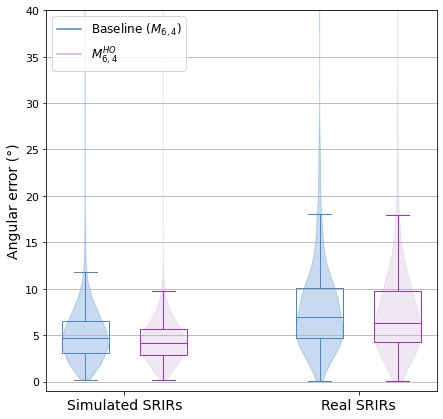
\includegraphics[width=.45\textwidth]{Images/chap7/boxplots_hoa_1src.png}\label{fig:boxplots_hoa_1src}}
    \subfloat[2-speaker signals]{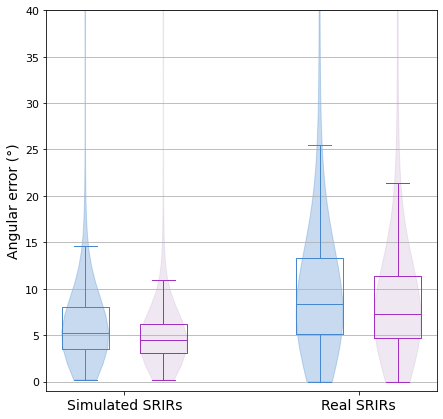
\includegraphics[width=.45\textwidth]{Images/chap7/boxplots_hoa_2src.png}\label{fig:boxplots_hoa_2src}}
    \subfloat[3-speaker signals]{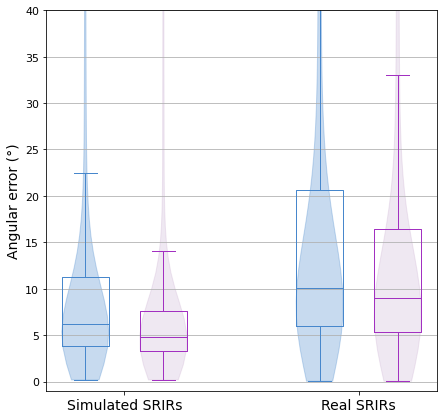
\includegraphics[width=.45\textwidth]{Images/chap7/boxplots_hoa_3src.png}\label{fig:boxplots_hoa_3src}}}
    
    \captionof{figure}[Boxplots of the angular errors of the model with HOA features and the baseline $M_{6,4}$ with FOA features on the simulated datasets]{Distribution of the angular error of the model with HOA features and the baseline with FOA features, evaluated on the test datasets $E^{Sim}_1$, $E^{Sim}_2$, $E^{Sim}_3$, $E^{Real}_1$, $E^{Real}_2$ and $E^{Real}_3$.}
    \label{fig:boxplots_multiLoca_hoa}
\end{figure}

\begin{figure}[t]
    \centering
    \begin{adjustbox}{width=1.3\textwidth,center}
        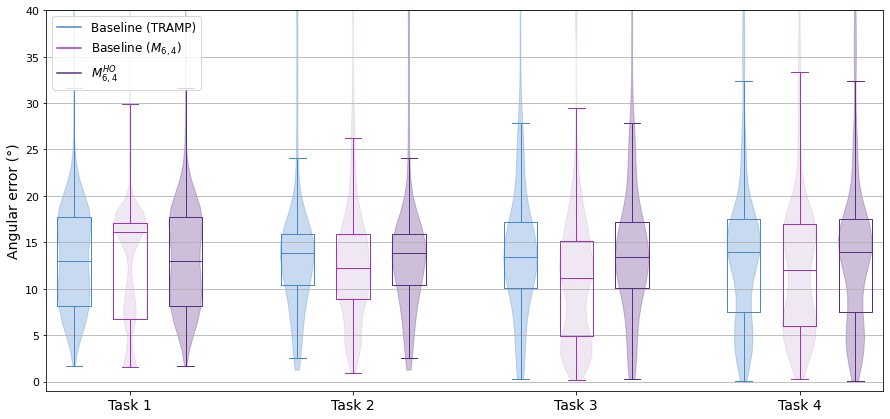
\includegraphics[width=1.\textwidth]{Images/chap7/boxplots_hoa_locata.png}
    \end{adjustbox}
    
    \captionof{figure}[Boxplots of the angular errors of the model with HOA features and the baselines with FOA features on the recorded dataset]{Distribution of the angular error of the model with HOA features and the baseline with FOA features, evaluated on the test datasets $E^{Rec}_1$, $E^{Rec}_2$, $E^{Rec}_3$ and $E^{Rec}_4$.}
    \label{fig:boxplots_multiLoca_hoa_locata}
\end{figure}

The results of this experiment are reported in Table~\ref{tab:multiLoca_hoa_results} and Fig.~\ref{fig:boxplots_multiLoca_hoa} and \ref{fig:boxplots_multiLoca_hoa_locata}. We can see that the model using HOA features surpasses the baseline with FOA features on the simulated datasets, however on real recordings the improvement is not conclusive. On the datasets $E^{Sim}_j$ and $E^{Real}_j$, the improvement is quite significant: the accuracy (< 10°) is increased from $95.3$\% (FOA features) to $98.8$\% (HOA features) on $E^{Sim}_1$, from $85.3$\% to $91.5$\% on $E^{Sim}_2$ and from $71.0$\% to $82.4$\% on $E^{Sim}_3$. On the datasets with real SRIRs, the improvement is similar (with all scores that are of course worse than on simulated data). We also observe that the gain in accuracy is better when there are more speakers, partly because the performance was already very high on $1$-speaker signals and quite good on $2$-speaker signals, but surely thanks to the better spatial resolution granted by the use of a HOA representation. This should give the network more information to better spatially separate the sources, therefore the benefit is emphasized when more sources are active. On real recordings, it is more difficult to assess the superiority of the HOA model. First, we see that the DNN-free baseline is better on $E^{Rec}_1$, which is not surprising since it is known to be performant on single-speaker signals. We observe a small improvement of the HOA model over the FOA model on the dataset $E^{Rec}_2$, with an accuracy of $73.1$\% against $70.3$\%, although the mean and median angular errors are higher. However, on the other multi-speaker dataset $E^{Rec}_4$, the HOA network shows worse results worse than the DL-based baseline.

Fig.~\ref{fig:output_visualization} shows an example of the outputs of the deep-learning-free baseline and the HO model $M^{HO}_{6,4}$ for one sequence of the test set $E^{Rec}_2$. We see that the baseline method leads to more scattered peaks than the neural network model, which could be detrimental to the localization performance if the sources are too close from each other. We notice that the network model outputs much more sparse values, however we notice a sort of ghost source, around $\theta=-100$ and $\phi=-40$, whose presence leads us to think that training the network only on $T_3$ forces it to output $3$ prominent peaks.

\begin{figure}[t]
    \centering
    \makebox[\textwidth][c]{
    \subfloat[TRAMP output]{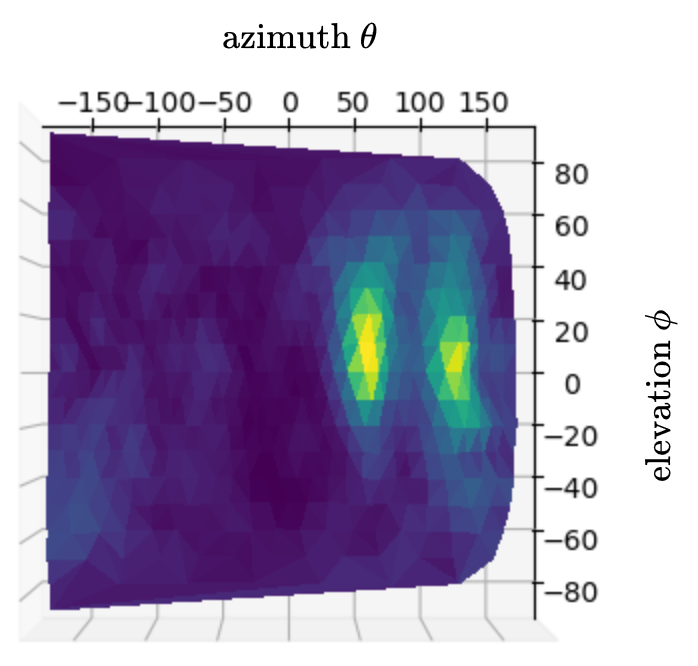
\includegraphics[width=.45\textwidth]{Images/chap7/tramp_hoa_plot.png}}
    \subfloat[$M^{HO}_{6,4}$ output]{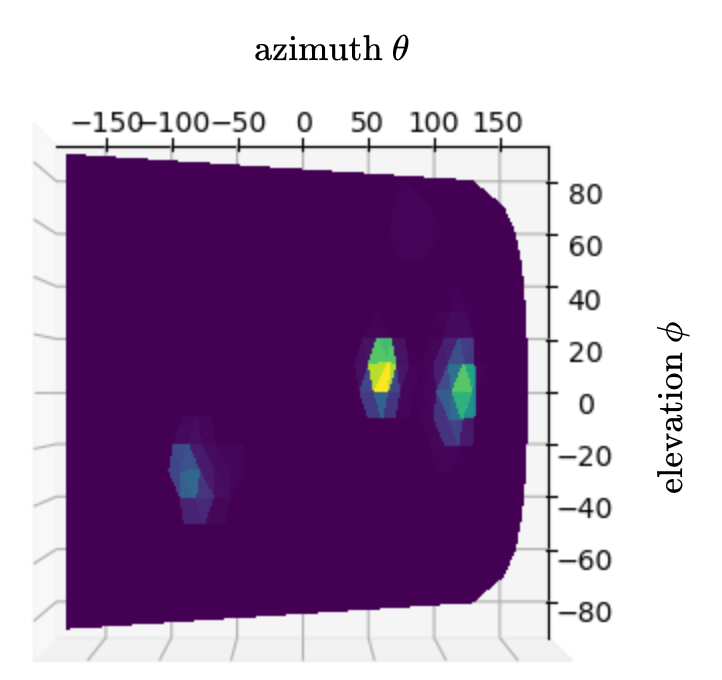
\includegraphics[width=.45\textwidth]{Images/chap7/dnn_hoa_plot.png}}}
    
    \captionof{figure}[Output DoA probability distributions of the TRAMP baseline and the HOA network]{Output DoA probability distributions of the TRAMP baseline (left) and the HOA network (right) on a sequence of the dataset $E^{Rec}_2$. Low values are represented with blue colors and high values with yellow colors.}
    \label{fig:output_visualization}
\end{figure}


\begin{table}[t]
\centering
    \subfloat[Simulated SRIRs]{
        \begin{adjustbox}{width=1.3\textwidth,center}
            \begin{tabular}{|c|cccc|cccc|cccc|}
            \hline
            \multirow{3}{*}{\textbf{Scenario}} & \multicolumn{4}{c|}{\textbf{$E^{Sim}_1$}}                                                          & \multicolumn{4}{c|}{\textbf{$E^{Sim}_2$}}                                                          & \multicolumn{4}{c|}{\textbf{$E^{Sim}_3$}}                                                           \\ \cline{2-13} 
                                                  & \multicolumn{2}{c}{\textbf{Accuracy (\%)}}       & \multicolumn{2}{c|}{\textbf{Angular error (°)}} & \multicolumn{2}{c}{\textbf{Accuracy (\%)}}       & \multicolumn{2}{c|}{\textbf{Angular error (°)}} & \multicolumn{2}{c}{\textbf{Accuracy (\%)}}       & \multicolumn{2}{c|}{\textbf{Angular error (°)}} \\
                                                  & \textbf{\textless{}10°} & \textbf{\textless{}15°} & \textbf{Mean}         & \textbf{Median}        & \textbf{\textless{}10°} & \textbf{\textless{}15°} & \textbf{Mean}         & \textbf{Median}        & \textbf{\textless{}10°} & \textbf{\textless{}15°} & \textbf{Mean}         & \textbf{Median}         \\ \hline
            FOA components only                          & 6.4                    & 13.6                    & 50.9                  & 36.0                    & 6.2                    & 13.1                    & 49.7                   & 38.2                    & 6.1                    & 12.3                    & 49.2                  & 38.8                     \\
            HOA components only  & 40.8           & 48.5          & 87.8          & 18.8           & 31.7           & 41.5           & 57.9          & 36.7           & 27.0           & 36.8           & 52.0        & 34.8            \\ \hline
            \end{tabular}
        \end{adjustbox}
    }
    
    \subfloat[Real SRIRs]{
        \begin{adjustbox}{width=1.3\textwidth,center}
            \begin{tabular}{|c|cccc|cccc|cccc|}
            \hline
                \multirow{3}{*}{\textbf{Scenario}} & \multicolumn{4}{c}{\textbf{$E^{Real}_1$}}                                                           & \multicolumn{4}{c}{\textbf{$E^{Real}_2$}}                                                           & \multicolumn{4}{c}{\textbf{$E^{Real}_3$}}                                                           \\ \cline{2-13} 
                                                      & \multicolumn{2}{c}{\textbf{Accuracy (\%)}}        & \multicolumn{2}{c|}{\textbf{Angular error (°)}} & \multicolumn{2}{c}{\textbf{Accuracy (\%)}}        & \multicolumn{2}{c|}{\textbf{Angular error (°)}} & \multicolumn{2}{c}{\textbf{Accuracy (\%)}}        & \multicolumn{2}{c|}{\textbf{Angular error (°)}} \\
                                                      & \textbf{\textless{}10°} & \textbf{\textless{}15°} & \textbf{Mean}         & \textbf{Median}        & \textbf{\textless{}10°} & \textbf{\textless{}15°} & \textbf{Mean}         & \textbf{Median}        & \textbf{\textless{}10°} & \textbf{\textless{}15°} & \textbf{Mean}         & \textbf{Median}        \\ \hline
                FOA components only                          & 4.5                    & 15.3                    & 51.9                   & 34.8                    & 5.3                    & 12.9                    & 50.6                  & 38.8                    & 5.6                    & 12.2                    & 51.3                  & 39.5                   \\
                HOA components only  & 31.6           & 43.8           & 86.3          & 33.4           & 25.3           & 36.0           & 63.6         & 41.8           & 23.2 & 33.8           & 58.1         & 43.1  
                \\ \hline
            \end{tabular}
        \end{adjustbox}
    }
    
    \captionof{table}[Accuracy and angular errors of the HOA model evaluated on signals with FOA components only and HOA components only]{Accuracy and angular errors of the HOA model evaluated on signals with FOA components only and HOA components only
    }
    \label{tab:hoa_model_flexibility_results}
\end{table}

For further analysis, we evaluate the model $M^{HO}_{6,4}$ on the test datasets for two additional configurations: when only the FOA components of the HO-PIV are kept, \emph{i.e.}, the other channels are forced to zero values, and when only the HOA components (order 2 in our case) are kept, \emph{i.e.}, the FOA channels are forced to zero values. The motivation for these experiments is to gain some insight in the way the network is using the Ambisonic features. Indeed, under certain hypothesis, the components of orders 1 and 2 can be used independently from one another to obtain an analytic DoA estimate.
The very low results in the first row of Table~\ref{tab:hoa_model_flexibility_results} first show that the network is not capable of relying only on FOA components when it has been trained with HOA features. This underlines that network characteristics of processing the features in its own specific manner to perform the learnt task. Moreover, we see that the results on the test datasets using only the HOA components are not as low as with FOA components only, it seems that the network finds more useful information in the components of order 2, than the FOA components. However, since the performance is much worse than when using all components, it is evident that the network has learnt how to efficiently combine features of all orders to perform the DoA estimation. This impressive combination capacity, which is not easily feasible analytically, underlines the general \textit{black box} characteristics of the neural networks, which we still have difficulties to fully understand today.

%-----------------------------------------------
%  CONCLUSION AND PERSPECTIVES
%-----------------------------------------------
\section{Conclusion and perspectives}

In this chapter, we addressed source localization when several speakers overlap in a noisy and reverberant mixture, and with the assumption of a known NoS. Based on the CRNN model proposed in \cite{perotin_crnn-based_2019}, we first questioned the optimal order in which we need to present the training examples to the network, which are made of $1$-, $2$- and $3$-speaker signals, to obtain the best performance. We found out that relying only on signals with $3$ speakers makes the network robust enough to perform well on mixtures with $1$ and $2$ speakers, whereas -- not surprisingly -- it is not capable of performing multi-speaker localization when trained only on $1$-speaker signals. Also, we understood that pretraining a localization network, followed by fine-tuning manner, \emph{i.e.}, with $1$-speaker signals first, then with $2$-speaker signals and finally with $3$-speaker signals, is not the best training scheme. We concluded that a good choice is to feed all examples randomly during the training phase, as it is done in most neural-based SSL systems.

Next, we proposed a redesign of the feature extraction module, made of convolutional and max-pooling layers, in an attempt to improve the multi-source localization performance of the baseline CRNN \cite{perotin_crnn-based_2019}. To give the network more capacity to extract its own meaningful features, we employed more convolutional layers and less aggressive max-pooling, leading to significantly more layers in total. We tried many models for a large set of hyperparameter values, and the results showed a significant improvement for all these models over the baseline, especially on mixtures with multiple speakers.

Then, we focused on replacing the recurrent layers usually employed in localization CRNNs with multi-head self-attention mechanism. The motivation was to dispose of recurrent layers, which are not parallelizable (and thus, \emph{e.g.}, limit the use of neural networks on embedded devices), as well as providing more flexibility in the temporal analysis with the self-attention mechanism. Using classical MHSA encoders, we managed to reach a similar localization performance as the CRNN baseline, with an inference time reduced by $44$\%. Furthermore, we improved the localization accuracy, especially in a multi-speaker context, by proposing a more general way of using several heads in the self-attention encoder.

Finally, we assessed the benefit of using a HO-PIV as an input feature for a CRNN. We obtained a substantial improvement on simulated datasets over the use of FO-PIV features, which was actually expected. However, on real recordings this improvement has not been observed, for reasons we do not understand. We also showed that such a network needs to use the components of all orders to successfully perform localization.

While significant improvements have been made over the baseline CRNN with the redesign of several neural modules, many aspects have not been treated in this research. First, the lack of in-depth analysis of our contributions makes it difficult to fully understand the obtained results. Regarding the new feature extraction module, although we intuit that more layers implies more network flexibility, it would be insightful to apply visualization techniques to interpret the behavior of convolutional layers. Among the available techniques to interpret the network computation, we can think of visualizing convolutional filter responses \cite[p~167]{chollet_deep_2017}, intermediate feature maps \cite[p.~160]{chollet_deep_2017} or using more advanced methods such as layer-wise propagation \cite{bach_pixel-wise_2015} as employed in \cite{perotin_localisation_2019}. In the same vein, analyzing the conduct of the self-attention mechanism and comparing it to the BiLSTM layers could give interesting insights on how the network processes a sequence in the temporal analysis module. Regarding these self-attention layers, it would also be interesting to apply these mechanisms in the frequency dimension, with the intuition that the attention heads could focus on the relation between specific frequency bins which contains the information of a specific speaker. This might gives more flexibility to the neural network to discriminate the different speakers using their spectral characteristics.  Moreover, our last experiment on HOA features could be carried on by first including all training data as done in the other methods, which would probably lead to better results not only on simulated data and but also on real recordings. Also, increasing the Ambisonics order, higher than $2$ as experimented here, should lead to an improvement in the localization performance, at the cost of much more data. Relying on a training dataset with directive sources could also be of interest \cite{gelderblom_synthetic_2021}. Again, an analysis on the network process over HO-PIV features could be very interesting, since it seems that the network has learnt some specific way of exploiting the first and second order features, different from analytical approaches. Finally, an idea we did not have time to experiment with is to think of a loss function which incorporates the NoS, as it is supposed to be known in these methods, in order to encourage the network to estimate the right number of DoAs. Practically, this could be done by forcing the network to output a spatial spectrum with the right number of peaks by penalizing it when additional high peaks are present in the output. This last idea is a first step towards combining speaker counting and localization, bringing us to the next chapter, which deals with this topic.